\documentclass[master]{finthesis}

\usepackage[babel, final]{microtype}
\usepackage{array}
\usepackage{extdash}
\usepackage{subcaption}
\usepackage{tikz}
    \usetikzlibrary{through, patterns}
\usepackage{multirow}
\usepackage{booktabs}
\usepackage{amsmath}

\addbibresource{main.bib}

\lstdefinestyle{Chisel}{
    language=Scala,
    morekeywords={abstract,case,catch,class,def,%
        do,else,extends,false,final,finally,%
        for,if,implicit,import,lazy,match,mixin,%
        new,null,object,override,package,%
        private,protected,requires,return,sealed,%
        super,this,trait,true,try,%
        type,val,var,while,with,yield,%
        when, elsewhen, otherwise, switch, is, it, should}, % Chisel "keywords"
    otherkeywords={=,=>,<-,<\%,<:,>:,\#,@,:,<>},
    escapechar={`}
}

\lstdefinelanguage{json}{
    string=[s]{"}{"},
    otherkeywords={:,[,],\{,\},\,},
}

\lstdefinelanguage{dirlist}{
    comment=[l]{.},
    otherkeywords={/},
    basicstyle=\ttfamily,
    commentstyle=\color{finComment}
}


\makeatletter
\newcommand*{\engl}[2][\@empty]{%
    \edef\theacronym{#1}%
    (енгл. \foreignlanguage{english}{\emph{#2}%
    \ifx\theacronym\@empty \else , #1\fi})%
}
\makeatother

\newcommand*{\kdim}[1]{\texorpdfstring{$k$\Hyphdash}{k-}димензионал#1}
\newcommand*{\kd}{\texorpdfstring{$k$}{k}-д }

\newcommand*{\correctmath}[1]{%
    \ifcsname mathCorrectionFor#1\endcsname%
        \csname mathCorrectionFor#1\endcsname%
    \else%
        #1%
    \fi%
}
\newcommand{\mathcorrection}[2]{\expandafter\newcommand\csname mathCorrectionFor#1\endcsname{#2}}
\mathcorrection{outPRom}{out\!P\!Rom}
\mathcorrection{addrPRom}{addr\!P\!Rom}
\mathcorrection{addrOutPRom}{addrOut\!P\!Rom}
\mathcorrection{p_addr}{p\_addr}
\mathcorrection{p_cnt}{p\_cnt}
\mathcorrection{checkIfPointCloser}{checkI\!f\!PointCloser}
\mathcorrection{leaf}{lea\!f}
\mathcorrection{performTest}{per\!f\!ormT\!est}
\mathcorrection{testWithGoldenModel}{testW\!ithGoldenM\!odel}
\mathcorrection{P_A}{P\_A}
\mathcorrection{tree_rom}{tree\_rom}
\mathcorrection{p_rom}{p\_rom}
\mathcorrection{pointElemWidth}{pointElemW\!idth}
\mathcorrection{log2Up}{log2U\!p}

\newcommand*{\mfield}[1]{{\langle\correctmath{#1}\/\rangle}}
\newcommand*{\field}[1]{\texorpdfstring{$\mfield{#1}$}{⟨#1⟩}}
\newcommand{\rv}{Ready\slash Valid}
\newcommand{\tabitem}{~~\llap{\textbullet}~~}
\newcommand*{\prog}[1]{\texttt{#1}}
\newcommand*{\op}[1]{\fbox{\prog{#1}}}
% \newcommand*{\func}[1]{$\correctmath{#1}$}
\newcommand*{\func}[1]{\prog{#1}}

\title{Хардверски акцелератор за алгоритам претраге најближег суседа унутар\texorpdfstring{\\}{ }\kdim{ног} стабла}
\author{Александар З. Кондић}
\studid{477/2019}
\advisor{проф. др Владимир М. Миловановић}
\advisorfull{Др Владимир М. Миловановић,\\ванредни професор}

\studprog{Електротехника и рачунарство}
% \module{Модул}
\course{Напредно машинско учење}
% \date{\today}
\date{2022-06-22}
\committee{проф. др Велибор Исаиловић}
\committee{доц. др Зоран Бабовић}

\studentshould{% У оквиру овог рада кандидат треба да...
    реализује хардверски акцелератор као решење проблема претраживања најближег суседа \kdim{не} тачке. Хардверска реализација алгоритма треба да се заснива на структури података \kdim{ног} стабла, која се складишти у меморији само за читање \engl{Read-only memory}. Решење треба да буде реализовано као генератор дигиталних модула помоћу Chisel обласно\Hyphdash специфичног језика \engl{Domain-specific language} за одговарајуће изабране улазне параметре. Генерисане примерке модула тестирати у оквиру софтверских симулација и верификовати њихову исправност на FPGA \engl{Field\Hyphdash programmable gate array} хардверској платформи. Спровести анализу искоришћења хардверских ресурса за различите примерке модула.
}

\titlepagebib{vahid2010digital}
\titlepagebib{chiselsite}

% Изгубили смо пријаву мастер рада, али студентска служба каже да није неопходна.
\renewcommand{\maketitle}{%
    \firsttitlepage%
    \secondtitlepage%
    \thirdtitlepage%
%     \fourthtitlepage%
}

\abstracten{
    A purpose of this thesis is to develop a digital hardware implementation of the nearest neighbour search algorithm (NNS) for \texorpdfstring{$k$}{k}-dimensional points. Searching for the nearest neighbour of a point involves finding a point from a predefined set of points with the smallest Euclidean distance from it. The search algorithm uses a \texorpdfstring{$k$}{k}-dimensional tree as a data structure that contains all predefined search points. Data about the points, as well as about the structure of the tree itself, are stored inside read-only memory (ROM). The solution is implemented as a digital hardware module generator by means of Chisel domain-specific language (DSL). Checking the correctness of the implementation is carried out through software simulations and hardware validation and verification.
}
\keywordsen{nearest neighbour search, \texorpdfstring{$k$}{k}-dimensional tree, read-only memory, software simulation, hardware validation and verification}

\abstractsr{
    Циљ овог \thesiscase{ог} рада је спровођење дигиталне хардверске реализације алгоритма за претраживање најближег суседа (NNS) \kdim{не} тачке. Претраживање најближег суседа неке тачке подразумева налажење тачке из унапред дефинисаног скупа тачака са најмањим еуклидским растојањем од ње. Алгоритам претраге користи \kdim{но} стабло као структуру података која садржи све унапред дефинисане тачке за претрагу. Подаци о тачкама, као и о структури самог стабла се складиште унутар меморије само за читање (ROM). Решење је реализовано као генератор дигиталних хардверских модула посредством Chisel обласно\Hyphdash специфичног језика (DSL). Провера исправности реализације спроводи се кроз софтверске симулације и хардверску валидацију и верификацију.
}
\keywordssr{претраживање најближег суседа, \kdim{но} стабло, меморија само за читање, софтверска симулација, хардверска валидација и верификација}

\begin{document}

\maketitle

\microtypesetup{protrusion=false}
\tableofcontents
\microtypesetup{protrusion=true}

\makeabstract

\section{Увод}

Претрага најближег суседа \engl[NNS]{Nearest Neighbour Search} је један од основних проблема статистичке класификације. Алгоритми за решавање овог, као и сличних проблема попут претраге $k$ најближих суседа имају примену у пољима вештачке интелигенције као што су машинско учење, рачунарска визија \cite{boiman2008defense} и роботика \cite{bewley2013advantages}. Суштина овог проблема је налажење тачке из предодређеног скупа тачака која је најближа улазној тачки.

Софтверска решења ових проблема већ постоје, међутим ради побољшања перформанси алгоритама разматрају се и хардверска решења. Алгоритми вештачке интелигенције се увелико извршавају на специјализованом хардверу направљеном само за ту намену \cite{talib2021systematic}. Хардвер који је посебно конструисан за решавање одређеног проблема на ефикаснији начин у поређењу са рачунарима опште намене и софтверским решењима зове се \emph{хардверски акцелератор}. Главна одлика хардверских акцелератора у односу на софтверска решења је њихова независност од процесора, односно \emph{централне процесорске јединице} \engl[CPU]{Central Processing Unit}, као јединог начина за спровођење операција над улазним подацима. У зависности од проблема који се решава, хардверски акцелератори могу имати висок степен паралелизације операција који није изводљив применом процесора опште намене, а самим тим и било ког софтвера, уколико није реч о специјализованим процесорима као што су \emph{графички процесори} \engl[GPU]{Graphics Processing Unit}.

Током реализације хардверског решења неког проблема неопходно је водити рачуна о ресурсима које тај хардвер користи. Ово се односи на број разних аналогних и дигиталних компоненти, површину коју они заузимају, као и њихов геометријски распоред у оквиру електронског кола које сачињавају. %Везано за проблем претраге најближег суседа тачке, један од главних проблема је одређивање начина на који се предодређени скуп тачака складишти на хардверу.
Пожељно је омогућити складиштење великог броја тачака са ефикасним искоришћењем хардверских ресурса. Најпогоднији начин за то је посредством меморијског модула. 

Дигитални меморијски модули садрже адресиране податке. Њима се приступа тако што се на улаз модула доведе вредност која представља адресу у меморији, а излаз модула буде податак који се налази на тој адреси. Једно ограничење оваквог приступа је то што је у једном циклусу такта доступан ограничен број података, који зависи од броја коришћених меморијских модула и количине података која се складишти на једном меморијском месту.

Да би се за неку улазну тачку одредила тачка која је њој најближа, неопходно је приступити свим тачкама одређеног подскупа скупа предодређених суседних тачака. С обзиром на то да је у једном циклусу такта доступан ограничен број тачака из тог скупа, пожељно је смањити број циклуса такта који је потребан да би се израчунао тачан резултат. Односно, потребно је смањити подскуп скупа предодређених тачака који садржи тачку која је најближа улазној. Ово ограничење је слично ограничењу софтверских решења, тако да је за оптимизацију решења овог проблема неопходно користити одговарајући алгоритам или структуру података.

\subsection{Специфичности реализације---дигитални хардвер,\texorpdfstring{\\}{ }платформа и алати}

Решење за овај проблем које се разматра заснива се искључиво на \emph{дигиталном} хардверу. Иако сваки дигитални хардвер по правилу треба да има и аналогне компоненте (кола за напајање, на пример), такве специфичности се овде не разматрају, углавном због природе платформе која је одабрана за реализацију дигиталног решења.

Циљна дигитална платформа за решење овог проблема је \emph{FPGA} \engl{Field Programmable Gate Array}. FPGA је чип који у себи садржи матрицу логичких блокова који могу да изврше функцију било ког логичког кола. Повезивањем ових блокова омогућује се прављење комбинационих кола. FPGA чипови у себи такође садрже меморијске елементе попут флип\Hyphdash флопова, регистара и меморијских модула, тако да је могуће правити и секвенцијална кола.

У суштини, FPGA чип у себи садржи такве елементе да је правилним подешавањем и повезивањем тих елемената могуће направити било које дигитално коло и реализовати произвољну дигиталну функцију. Дигитално коло на FPGA платформи се реализује тако што се при напајању FPGA чип програмира, односно дефинише се шема логичких блокова који се користе и њихове функције, као и начин на који су ти блокови повезани међусобно и са осталим елементима чипа попут меморијских блокова. Шема по којој се ова подешавања спроводе дефинише корисник платформе у неком од специјализованих алата за ту намену.

Најчешћи начин пројектовања дигиталног кола је коришћењем \emph{језика за опис хардвера} \engl[HDL]{Hardware Description Language} \cite{vahid2010digital}. HDL језици као што су VHDL \cite{ieee1076-2019} и Verilog \cite{ieee1800-2017} се заснивају на RTL \engl{Register Transfer Level} апстракцији дизајна, преко које се дигитално коло моделира као скуп логичких операција над улазним дигиталним сигналима и хардверских регистара у којима се чувају резултати тих операција.

Постоје разна дигитална хардверска решења алгоритама вештачке интелигенције. Неки од тих решења баш користе RTL језике као што су VHDL и Verilog \cite{mohsin2018fpga}, \cite{ito2018nearest}. Међутим, колико год да су наведени језици за опис хардвера погодни за дигитално пројектовање, они имају и своја ограничења. Та ограничења се углавном односе на недовољно флексибилну могућност параметризације дизајна---тј. да се посредством параметара утиче на структуру хардверског модула---као и недостатак језичких конструкција вишег нивоа које су присутне у програмским језицима, нпр. функције, конструкције за једноставно исказивање сложенијих аритметичких операција и др. Један начин да се заобиђу ова ограничења је посредством \emph{генератора RTL кода}. Генератори су програми који генеришу RTL код у неком од HDL језика. Генератори се углавном пишу у неком од програмских језика вишег нивоа (нпр. Пајтон, Скала, итд.). Овај \thesiscase{и} рад разматра решење које је написано као генератор у \emph{Chisel} \cite{bachrach2012chisel} обласно\Hyphdash специфичном језику \engl[DSL]{Domain-specific language}.

Chisel је дефинисан као језик за опис хардвера \cite{chiselsite}. Реализован је као библиотека за програмски језик Скала \engl{Scala} \cite{scalasite} која јој додаје примитиве за конструисање дигиталног хардвера. Код написан у Chisel-у чини генератор RTL кода у HDL језику попут Verilog-а. Предност у коришћењу Скале и Chisel-а се огледа у могућности коришћења језичких конструкција Скале и могућности параметризације које пружа Chisel при писању RTL кода. На пример, могу се користити конструкције функционалних и објектно-оријентисаних програмских језика, које пружа Скала. Параметризација генератора се такође врши на нивоу програмског језика Скале---посредством Chisel-а---преко које се одређује које Chisel примитиве се користе за конструкцију хардвера на основу вредности улазних параметара.

Chisel као библиотека такође пружа могућност софтверске симулације написаних модула. Могу да се дефинишу тестови који симулираном модулу прослеђују улазне податке и испитују тачност излазних података модула. Симулација се заправо спроводи у посебном програму за симулацију дигиталних модула, са којим Chisel одржава комуникацију---прослеђује му изгенерисан RTL код и улазне сигнале, чита излазне сигнале из симулатора и пореди их са очекиваним вредностима дефинисаним у тестовима, итд. Ова функционалност реализована је као посебна Chisel-ова библиотека звана ChiselTest. Неки од екстерних програма који се користе за симулирање дигиталних кола су Treadle и Verilator \cite{chiseltest}.

HDL језик за који се генерише RTL код из Chisel генератора у оквиру овог \thesiscase{ог} рада је Verilog. За претварање изгенерисаног Verilog кода у шему која се користи за подешавање FPGA чипа користи се Xilinx Vivado \cite{vivadosite}. За развој FPGA чипа такође се користи FPGA развојна плоча. Конкретна плоча на којој је реализовано решење датог проблема у оквиру овог \thesiscase{ог} рада је Digilent Arty A7 \cite{arty7site} са Xilinx Artix-7 FPGA фамилијом чипова \cite{artix7site}.

\section{Претраживање најближег суседа}

Најједноставнији начин да се за улазну тачку нађе њен најближи сусед из предодређеног скупа тачака $P$ је да се спроведе линеарна претрага кроз скуп $P$. За сваку тачку из скупа се рачуна њено растојање од улазне тачке и бележи се тачка која има тренутно најмање растојање од улазне тачке. Овакав алгоритам има линеарну временску сложеност---ако је $n$ број тачака из скупа $P$, временска сложеност алгоритма је $\mathcal{O}(n)$. Међутим, да би се некој улазној тачки нашао најближи сусед, није неопходно испитати цео скуп $P$. Пожељно би било смањити геометријски простор претраге тачака на део простора који садржи улазну тачку и предодређене тачке које су у њеној релативној близини.

Простор који заузимају тачке из скупа $P$ може се поделити на више потпростора, а претрага да се ограничи на потпросторе који су најближи улазној тачки. Једна од метода поделе простора је \emph{бинарна подела простора} \engl{binary space partitioning}. Ова метода рекурзивно дели простор на два потпростора, где се подела врши преко хиперравни. Тачке које се налазе са супротних страна хиперравни припадају различитим потпросторима. Ово је општа метода поделе простора, а конкретне методе се разликују по томе како дефинишу хиперраван која дели простор на два дела, и по критеријуму за престанак даље рекурзивне поделе. Методе бинарне поделе простора имају примену у рачунарској графици \cite{fuchs1980visible}.

Једна од метода бинарне поделе простора је коришћење структуре података \kdim{ног} стабла, скраћено \kd стабла. \kdim{но} стабло је тип бинарног стабла претраге код којег чворови садрже \kdim{не} тачке. Сваки чвор у стаблу представља један (под)простор. Деца чвора у стаблу представљају његове потпросторе подељене одговарајућом хиперравни.

Даље следи детаљнији опис структуре \kd стабла, као и начин на који се врши претраживање тачака кроз стабло.

\subsection{Структура \kdim{ног} стабла}

Хиперраван која дели простор који припада одређеном чвору \kdim{ног} стабла се дефинише на следећи начин. Бира се једна од координата тачке у чвору. Хиперраван је онда дефинисана као геометријско место тачака код којих су вредности одабране координате једнаке вредности координате тачке у чвору. То ефективно значи да за одређену координату тачке у чвору, свака тачка у простору која има мању вредност одговарајуће координате припада левом подстаблу, а свака тачка која има већу вредност одговарајуће координате припада десном подстаблу. За сврху претраживања најближег суседа, тачка која има исту вредност одговарајуће координате (припада хиперравни) може да припада било ком од два подстабала\slash потпростора.

Координата тачке по којој се простор дели на два потпростора зависи од дубине у стаблу чвора којем припада. Одређује се редослед координата по којем се врши подела простора. Како се пролази кроз стабло његовом дубином, координате по којима се дели простор се мењају по датом редоследу. За чворове стабла чије су дубине веће од броја димензија тачака овај редослед се периодично понавља. Редослед координата по којем се дели простор углавном одговара редоследу координата које се задају при дефинисању неке \kdim{не} тачке. Рекурзивно дељење простора се завршава када он садржи само једну тачку---такви простори припадају листовима \kd стабла.

Решење разматрано у овом \thesiscase{ом} раду користи другачију варијанту \kdim{ног} стабла. Једна од разлика је та да листови стабла представљају потпросторе који у себи могу да имају више од једне тачке, тј. у тим потпросторима је заустављена даља рекурзивна подела. Другим речима, листови \kd стабла могу да садрже једну или више тачака. Када се током претраге стабла посети лист, његове тачке се редом претражују, односно спроводи се линеарна претрага.

Друга разлика коришћене варијанте \kd стабла се огледа у садржају чворова стабла који нису листови. Они не садрже тачке, него само вредности одговарајуће координате по којој се врши подела простора у том чвору. Код ове варијанте \kd стабла, све тачке се налазе искључиво у листовима. Вредност координате по којој се врши подела простора одговара вредности исте координате једне од тачака.

На слици~\ref{fig:kdfig} дат је пример \kdim{ног} стабла где је $k = 2$. На слици се могу видети хоризонталне и вертикалне праве које деле дводимензионални простор на потпросторе. Свакој правој припада бар по једна тачка. Корен стабла представља целокупни простор тачака. Тачке чије су вредности $X$ координате мање или једнаке $4$ се налазе у левом подстаблу и припадају левом потпростору, док обрнуто важи за тачке чије су вредности $X$ координате веће од $4$.

\begin{figure}[h]
    \includegraphics[width=\linewidth]{slike/kd_fig}
    \caption{Пример дводимензионалног ($k = 2$) стабла.}
    \label{fig:kdfig}
\end{figure}

Раније је напоменуто да за потребе претраге најближег суседа, тачка која припада хиперравни која дели простор може да припада било ком од два потпростора. У овом раду је та чињеница искоришћена за конструисање балансираног \kd стабла из скупа предодређених тачака. Најпре се одреди дубина стабла. Онда се за скуп предодређених тачака нађе вредност медијане прве координате. Прави се чвор који представља корен стабла и он садржи вредност медијане. Све тачке чије су вредности одговарајуће координате мање од медијане иду у лево подстабло, док тачке чије су вредности одговарајуће координате веће од медијане иду у десно подстабло. Тачке чије су вредности одговарајуће координате једнаке медијани се деле на лево и десно подстабло тако да се бројеви тачака у њима разликују највише за један. Ова процедура се рекурзивно извршава у левом и десном подстаблу док се не постигне жељена дубина стабла.

У дигиталној реализацији разматраног решења подаци \kdim{ног} стабла се складиште у две меморије само за читање (два ROM-а). Садржаји ових меморија су одређени током програмирања FPGA чипа и они се не могу променити током његовог рада. Један ROM садржи податке о структури \kd стабла, док други садржи предодређене тачке. На слици~\ref{fig:kdroms} приказана је шема по којој су организовани подаци у меморијама за \kd стабло одређене структуре. Меморија која садржи структуру стабла означена је са ,,Tree ROM,'' а меморија која садржи тачке означена је са ,,Points ROM.'' 

\begin{figure}[h]
    \includegraphics[width=\linewidth]{slike/kd_roms}
    \caption{Изглед меморијске шеме \kd стабла.}
    \label{fig:kdroms}
\end{figure}


У \kdim{ном} стаблу на слици~\ref{fig:kdroms} вредности у чворовима нису вредности медијане (под)скупова тачака. Вредности у чворовима, ради илустрације, заправо представљају индексе, односно адресе, тих чворова у Tree ROM-у. За овакво дефинисано индексирање чворова важи да уколико је индекс неког чвора у стаблу $n$, индекси његовог левог и десног детета су редом $2n + 1$ и $2n + 2$.

Поља сваког елемента у Tree ROM-у су редом: \field{leaf}, \field{value}, \field{p_addr}, и \field{p_cnt}. Свако поље на слици~\ref{fig:kdroms} означено знаком $\times$ нема валидну вредност. Следи опис сваког од наведених поља:
\begin{description}
    \item[\field{leaf}] Индикатор који одређује да ли је чвор лист стабла. Вредност $0$ означава да није, док вредност $1$ означава да јесте. Када је вредност овог поља једнака $0$, вредности поља \field{p_addr} и \field{p_cnt} нису валидне. Када је вредност овог поља једнака $1$, вредност поља \field{value} није валидно.
    
    \item[\field{value}] Вредност одговарајуће координате на основу које се врши подела простора на два потпростора. У случају овог рада та вредност је увек једнака медијани неког од подскупова скупа предодређених тачака. Вредност овог поља се користи само код чворова стабла који нису листови.

    \item[\field{p_addr}] Почетна адреса у Points ROM-у скупа тачака који припада чвору. Вредност овог поља се користи само код чворова стабла који су листови. Тачке у Points ROM-у су организоване тако да све тачке које припадају једном листу стабла имају узастопне адресе.

    \item[\field{p_cnt}] Број тачака који припада чвору стабла. Вредност овог поља се користи само код чворова стабла који су листови.
\end{description}

Поља $\mfield{p_0}, \mfield{p_1}, \dots, \mfield{p_{k-1}}$ у Points ROM-у представљају вредности одговарајућих координата тачака. Као што је напоменуто, тачке које припадају истом листу \kd стабла заузимају узастопна места у меморији.

\subsection{Алгоритам претраживања}

Алгоритам претраживања најближег суседа рекурзивно претражује \kdim{но} стабло кроз његову дубину. Његов рад је сличан раду алгоритма претраге у дубину \engl[DFS]{Depth-first search}, те се може рећи да је он једна од његових варијација.

Алгоритам претраге у дубину је општи алгоритам претраге графова који може да се примени и на бинарно стабло пошто је стабло специјалан случај графа. Почевши од корена стабла, редом се посећују његова деца. Када се дође до чвора детета, исти процес се понавља, посећујући редом и његову децу. Када чвор нема децу, алгоритам се враћа на његовог родитеља и посећују се остала деца родитеља.

Алгоритам претраге у дубину, када се посећује неки чвор стабла, за свако дете чвора редом позива нову инстанцу истог алгоритма. Алгоритам дубинске претраге је стога рекурзиван. То значи да се друго дете неког чвора неће посећивати док DFS потпуно не обиђе прво дете. Пошто исто важи и за посећивање деце првог детета, претрага у дубину ће кренути да посећује друго дете чвора тек када се посете сви чворови у подстаблу чији је корен прво дете чвора.

Што се тиче редоследа којим се посећују деца, он код DFS алгоритма није од значаја пошто је једна од намена претраге у дубину да се обиђе цео подграф који почиње у датом чвору. Код бинарних стабала, постоје две могућности: лево дете, па десно, или десно дете, па лево. На слици~\ref{fig:dfs} дат је пример рада DFS алгоритма. На врху је дат пример једног бинарног стабла, а испод је назначен редослед којим се чворови обилазе приликом претраге стабла у дубину. Редослед обиласка деце чворова је прво лево дете, па онда десно. На слици се може приметити како се алгоритам враћа на родитеља чвора чији је обилазак завршен, након чега се наставља процес обиласка родитеља онде где је био заустављен у тренутку када се прешло на обилажење његовог детета.

\begin{figure}[ht]
    \centering
    \includegraphics[height=0.6\textheight]{slike/dfs_traversal}
    \caption{Пример претраге бинарног стабла у дубину.}
    \label{fig:dfs}
\end{figure}

Алгоритам претраживања најближег суседа у оквиру \kdim{ног} стабла је сличан DFS-у, уз пар разлика. Прво, редослед по којем се посећују деца чвора није произвољан, него зависи од улазне тачке за коју се тражи најближи сусед. За тренутни чвор стабла се узима у обзир вредност координате по којој се дели простор. Онда се вредност одговарајуће координате улазне тачке пореди са том вредношћу и претраживање се наставља у подстаблу који одговара потпростору у којем се налази улазна тачка. Прво дете чвора које се обилази је оно чијем простору припада тачка за коју се тражи најближи сусед. Када се евентуално дође до листа стабла, исцрпно се пролази кроз све тачке у том чвору и бележи се која је тачка најближа улазној тачки. Онда се претрага враћа на родитеља тог листа стабла.

Друга разлика између претраживања најближег суседа и DFS-а је та што код претраживања најближег суседа није загарантовано да ће се за неки чвор обилазак извршити за оба његова детета. Када се, након обиласка његовог првог детета претраживање врати на тренутни чвор, одлучује се да ли је неопходно извршити обилазак другог детета. То се чини само у случају када у простору који припада другом детету чвора може постојати тачка која је ближа улазној тачки од тренутно најближе. Односно, уколико хиперсфера, са центром у улазној тачки и дужином полупречника која је једнака растојању тренутно најближе тачке од улазне тачке, сече хиперраван која дели простор на два дела, онда део хиперсфере са друге стране хиперравни може садржати тачке из тог потпростора са мањим растојањем од улазне тачке него што је дужина полупречника хиперсфере.

У практичном смислу, за тренутни чвор се рачуна минимално растојање улазне тачке од његове хиперравни која дели простор, и то растојање се пореди са растојањем тренутно најближе тачке улазној тачки. Уколико је растојање улазне тачке од хиперравни мање од растојања њој тренутно најближе тачке, посећује се и потпростор са супротне стране хиперравни у потрази за потенцијално ближим тачкама улазној тачки.

На слици~\ref{fig:hypersphere} може се видети илустрација овог одлучивања у две димензије. Хиперраван $p$ је представљена испрекиданом линијом која дели дводимензионални простор на леви и десни потпростор. Тачка $U$ представља улазну тачку, док је тачка $M$ њој тренутно најближа тачка. Кругом је представљена хиперсфера са центром у тачки $U$ и полупречником једнаком растојању тачке $M$ од тачке $U$. Тачка $N$ се налази са друге стране хиперравни у потпростору који још увек није претражен. На слици~\ref{fig:hypersphere:nobreach} тачка $M$ је ближа улазној тачки него хиперраван $p$. У том случају се неће посећивати десни потпростор. У случају слике~\ref{fig:hypersphere:breach} хиперраван $p$ је ближа тачки $U$, што значи да у десном потпростору можда постоји тачка која је ближа тачки $U$ него тачка $M$. Претрага се наставља у десном потпростору и евентуално се наилази на тачку $N$ која постаје нова тренутно најближа тачка улазној тачки $U$.

\begin{figure}[ht]
    \begin{subfigure}[b]{0.48\linewidth}
        \centering
        \begin{tikzpicture}
            \coordinate [label=above:$U$] (U) at (3,3);
            \coordinate [label=left:$M$] (M) at (2,2);
            \coordinate [label=right:$N$] (N) at (5.5,3.5);
            \draw[dashed] (5, 0) -- (5, 6) node[anchor=north west] {$p$};
            \node [draw] at (U) [circle through={(M)}] {};
            \draw (U) -- (M);
            \foreach \Point in {(U), (M), (N)}{
                \fill \Point circle[radius=2pt];
            }
        \end{tikzpicture}
        \caption{Тачка $M$ је ближа улазној тачки него хиперраван $p$.}
        \label{fig:hypersphere:nobreach}
    \end{subfigure}
    \hfill
    \begin{subfigure}[b]{0.48\linewidth}
        \centering
        \begin{tikzpicture}
            \coordinate [label=above:$U$] (U) at (4,3);
            \coordinate [label=left:$M$] (M) at (2,2);
            \coordinate [label=right:$N$] (N) at (5.5,3.5);
            \draw[dashed] (5, 0) -- (5, 6) node[anchor=north west] {$p$};
            \node [draw] at (U) [circle through={(M)}] {};
            \draw (U) -- (M);
            \foreach \Point in {(U), (M), (N)}{
                \fill \Point circle[radius=2pt];
            }
        \end{tikzpicture}
        \caption{Хиперраван $p$ је ближа улазној тачки него њој тренутно најближа тачка $M$.}
        \label{fig:hypersphere:breach}
    \end{subfigure}

    \caption{Илустрација хиперравни~$p$ која дели простор (испрекидана линија) и хиперсфере (круг) са центром у улазној тачки~$U$ која садржи њој тренутно најближу тачку~$M$.}
    \label{fig:hypersphere}
\end{figure}

Пример проласка алгоритма претраживања најближег суседа кроз \kdim{но} стабло дат је на слици~\ref{fig:kd-traversal}. Испод стабла дат је редослед посећивања његових чворова од стране NNS алгоритма. Изнад сваког чвора налази се кратка илустрација о операцијама које се извршавају током његовог посећивања. Алгоритам се извршава за улазну тачку $(5, 3)$. Растојања су квадратна. Даље следи кратак опис корака који су предузети током посећивања чворова у датом примеру:
\begin{description}
    \newcommand*{\nonleaf}[1]{\item[{%
        \tikz[anchor=south,baseline=4pt] \draw node[align=center,draw,circle] {#1};%
    }]}
    
    \newcommand*{\nl}{\\\hline}
    \newcommand*{\leaf}[1]{\item[{%
        \tikz [anchor=south,baseline=5pt] \draw node {\hspace{-5pt}\begin{tabular}{|>{\centering\arraybackslash}p{3em}|}\hline #1\nl\end{tabular}};%
    }]}
    
    \nonleaf{$4$} $X$ координата улазне таче ($5$) није мања од вредности у чвору ($4$), претраживање се наставља у десном подстаблу.
    \nonleaf{$6$} $Y$ координата улазне тачке ($3$) је мања од вредности у чвору ($6$), претраживање се наставља у левом подстаблу.
    \leaf{$(8, 3)$\nl$(14, 16)$} Нова најближа тачка улазној тачки је $(8, 3)$. Квадратно растојање тренутно најближе тачке од улазне тачке је $9$. Претраживање се враћа на родитеља.
    \nonleaf{$6$} Квадратно растојање улазне тачке од хиперравни је $9$. Пошто то растојање није мање од растојања тренутно најближе тачке од улазне тачке ($9$), прескаче се друго дете. Претраживање се враћа на родитеља.
    \nonleaf{$4$} Квадратно растојање улазне тачке од хиперравни је $1$, што је мање од квадратног растојања тренутно најближе тачке од улазне тачке ($9$). Потребно је претражити друго дете.
    \nonleaf{$3$} $Y$ координата улазне тачке ($3$) није мања од вредности у чвору ($3$), претраживање се наставља у десном подстаблу.
    \leaf{$(2, 12)$\nl$(4, 13)$\nl$(3, 14)$} Није пронађена ближа тачка улазној од тренутне најближе. Претраживање се враћа на родитеља.
    \nonleaf{$3$} Квадратно растојање улазне тачке од хиперравни је $0$, што је мање од квадратног растојања тренутно најближе тачке од улазне тачке ($9$). Потребно је претражити друго дете.
    \leaf{$(2, 2)$\nl$(3,3)$} Нова најближа тачка улазној тачки је $(3, 3)$. Квадратно растојање тренутно најближе тачке од улазне тачке је $4$. Претраживање се враћа на родитеља.
    \nonleaf{$3$} Оба детета су претражена. Претраживање се враћа на родитеља.
    \nonleaf{$4$} Оба детета су претражена. Крај.
\end{description}

% Ново 2: Временска сложеност алгоритма
\smallskip
Уколико су $N$ број чворова у \kd стаблу и $M$ број тачака по листу стабла, очекивана временска сложеност алгоритма претраживања најближег суседа је $\mathcal{O}(\log_2\!N + M)$. Да би се од корена стабла стигло до листа потребно је $\mathcal{O}(\log_2\!N)$ операција, док је за исцрпну претрагу тачака у листу потребно $\mathcal{O}(M)$ операција. Да би сложеност алгоритма остала логаритамска, пожељно је да $M$ увек буде мања или једнака некој константној вредности $l$. У том случају би број чворова у стаблу зависио од броја тачака, односно за број тачака у стаблу $P$, број чворова у стаблу би био $$N \approx \frac{P}{M} \ge \frac{P}{l}.$$ У том случају, временска сложеност извршавања алгоритма претраживања најближег суседа у односу на број тачака у стаблу је $$\mathcal{O}(\log_2\!N + M) = \mathcal{O}(\log_2\!\frac{P}{M} + M) = \mathcal{O}(\log_2\!P).$$ Претпоставка је да је вредност променљиве $M$ ограничена неједнакошћу $M \le l$ где је $l$ константа, те се $M$ рачуна као константан фактор у асимптотској временској сложености алгоритма.

Дата анализа временске сложености се односи на очекивану или просечну сложеност. Временска сложеност умногоме зависи од дистрибуције тачака у \kd стаблу, као и од позиције тачке којој треба да се нађе најближи сусед. У најгорем случају, временска сложеност алгоритма претраживања најближег суседа у \kdim{ном} стаблу је ипак $\mathcal{O}(N + M)$, тј. $\mathcal{O}(P)$ уколико је $M$ мања или једнака константи $l$. Односно, временска сложеност алгоритма је у најгорем случају линеарна, што у том случају алгоритму не даје знатну предност у односу на исцрпну претрагу свих тачака у стаблу.

\begin{figure}
    \centering
    \includegraphics[height=0.9\textheight]{slike/kd_traversal_sr.pdf}
    \caption{Пример проласка NNS алгоритма кроз \kd стабло.}
    \label{fig:kd-traversal}
\end{figure}

Најгори случај у раду алгоритма претраживања најближег суседа у оквиру \kd стабла може да се постигне када је растојање најближе тачке од дате тачке веће од растојања дате тачке од већине потпростора које представљају чворови \kd стабла. Неки од примера таквих случајева су када је тачка за коју треба да се нађе најближи сусед на великом растојању од свих тачака у \kd стаблу, и када су тачке унутар стабла распоређене приближно у облику хиперсфере, а улазна тачка се налази у близини њеног центра. У оба случаја су тачке у \kd стаблу приближно једнако удаљене од тачке за коју је потребно наћи најближи сусед.

На слици~\ref{fig:worstcase} може се видети приказ наведених најгорих случајева за рад NNS алгоритма у дводимензионалном стаблу. Хоризонталне и вертикалне испрекидане линије означавају поделе у простору. Кругови на слици имају центре у улазној тачки $U$ и садрже њој најближу тачку $M$. Правоугаоници састојани из испрекиданих линија, који не садрже друге такве правоугаонике, представљају појединачне потпросторе сваког листа у \kd стаблу.

На слици~\ref{fig:worstcase:faraway} приказан је случај када је улазна тачка знатно удаљена од тачака у \kd стаблу. У овом случају, хоризонталне и вертикалне удаљености улазне тачке од одговарајућих равни које деле дводимензионални простор су мање од удаљености њој најближе тачке из стабла. У случају слике~\ref{fig:worstcase:center}, тачке у стаблу су распоређене у кругу са центром у улазној тачки. У овом случају, већине подела у потпросторима се дешавају у околини улазне тачке на удаљености мањој од удаљености њој најближе тачке. На слици је осенчен једини потпростор који се неће посећивати при претраживању најближег суседа улазној тачки $U$.

\begin{figure}[ht]
    \begin{subfigure}[t]{0.48\linewidth}
        \centering
        \begin{tikzpicture}[x=0.078\linewidth, y=0.078\linewidth]
            \coordinate [label=above:$U$] (U) at (-9,10);
            \coordinate [label=left:$M$] (M) at (0,3);
            
            \draw[dashed] (1,  0) -- (1, 10);
            
            \draw[dashed] (-9, 1) -- (3,  1);
            
            \draw[dashed] (0,  0) -- (0, 10);
            \draw[dashed] (2,  0) -- (2, 10);

            \draw[dashed] (-9, 0) -- (3,  0);
            \draw[dashed] (-9, 2) -- (3,  2);

            % \fill[pattern=north east lines] (0,0) rectangle (3,2);
            
            \draw ([shift={(0:11.4018)}]U) arc(0:-62:11.4018);
            \draw (U) -- (M);
            
            \foreach \x in {0,...,3}
                \foreach \y in {0,...,3}
                    {\fill (\x,\y) circle[radius=2pt];}
            \fill (U) circle[radius=2pt];
        \end{tikzpicture}
        \caption{Тачка~$M$ је најближа улазној тачки~$U$, али то растојање је веће од растојања тачке~$U$ од хиперравни које деле простор.}
        \label{fig:worstcase:faraway}
    \end{subfigure}
    \hfill
    \begin{subfigure}[t]{0.48\linewidth}
        \centering
        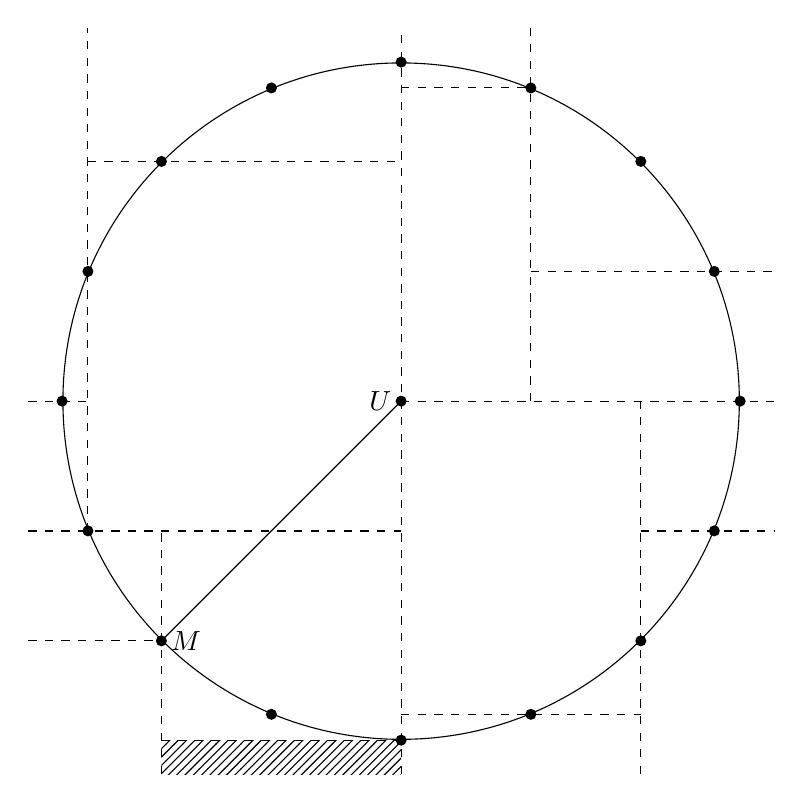
\begin{tikzpicture}[x=0.0355\linewidth, y=0.0355\linewidth]
            \draw[dashed] (0, -11) -- (0, 11);

            \draw[dashed] (-11, -3.83) -- (0, -3.83);
            \draw[dashed] (0, 0) -- (11, 0);

            \draw[dashed] (-7.07, -11) -- (-7.07, -3.83);
            \draw[dashed] (-9.24, -3.83) -- (-9.24, 11);
            \draw[dashed] (7.07, -11) -- (7.07, 0);
            \draw[dashed] (3.82, 0) -- (3.82, 11);

            \draw[dashed] (-11, -7.07) -- (-7.07, -7.07);
            \draw[dashed] (-7.07, -10) -- (0, -10);
            \draw[dashed] (-11, 0) -- (-9.24, 0);
            \draw[dashed] (-9.24, 7.07) -- (0, 7.07);
            \draw[dashed] (0, -9.24) -- (7.07, -9.24);
            \draw[dashed] (7.07, -3.83) -- (11, -3.83);
            \draw[dashed] (0, 9.24) -- (3.83, 9.24);
            \draw[dashed] (3.83, 3.83) -- (11, 3.83);

            \foreach \i in {0,...,15} {
                \coordinate (A\i) at (\i*360/16:10);
                \fill (A\i) circle (2pt);
            }
            
            \coordinate [label=left:$U$] (U) at (0, 0);
            \coordinate [label=right:$M$] (M) at (A10);
            \fill (U) circle[radius=2pt];

            \draw (U) -- (M);
            \node [draw] at (U) [circle through={(M)}] {};

            % \fill[pattern=north east lines] (-11, -11) rectangle (-7.07, -7.07);
            \fill[pattern=north east lines] (-7.07, -11) rectangle (0, -10);
        \end{tikzpicture}
        \caption{Тачке у стаблу су распоређене у кругу са центром у улазној тачки~$U$. Осенчени правоугаоник представља једини потпростор који се неће посећивати.}
        \label{fig:worstcase:center}
    \end{subfigure}

    \caption{Илустрација најгорих случајева за рад NNS алгоритма у дводимензионалном ($k = 2$) простору.}
    \label{fig:worstcase}
\end{figure}

\section{Хардверска реализација алгоритма}

Као што је већ напоменуто, хардверско решење овог проблема реализовано је у Chisel-у као параметризовани генератор Verilog кода који генерише различите хардверске модуле за претраживање \kd стабла на основу вредности улазних параметара. Реализација је отвореног кода и јавно је доступна за коришћење као хардверска библиотека \cite{kondic2022hardware}.

Алгоритам претраживања најближег суседа је рекурзиван. Софтверске реализације овог алгоритма могу да буду у облику рекурзивне функције, где се рекурзија остварује преко позивног стека. Алтернативно се алгоритам може реализовати као класична функција која експлицитно користи стек структуру података за складиштење чворова за посећивање. У дигиталној хардверској реализацији рекурзивних алгоритама неопходно је---уколико се алгоритми не могу трансформисати у итеративне---експлицитно користити стек структуру података. У оквиру разматраног решења тај стек је реализован као низ регистара фиксне дужине која представља максималну дубину стека, са још једним регистром који показује на врх стека.

Параметри генератора се односе на улазне и излазне сигнале, на структуру \kdim{ног} стабла и тачака које су у њему садржане. Пошто је структура стабла дефинисана искључиво преко ROM-ова са слике~\ref{fig:kdroms}, параметризација се онда, поред улазних и излазних сигнала, односи на структуру наведених меморија. Поред броја меморијских места у сваком ROM-у може да се параметризује и ширина у битовима поља ROM-ова. У наставку су дати параметри генератора дефинисани у разматраном решењу проблема:
\begin{description}
    \item[\field{pointNumDimensions}] Број димензија тачака у стаблу. Поред улазних и излазних сигнала, овај параметар одређује и број поља сваког елемента у Points ROM-у.
    \item[\field{treeDepth}] Дубина \kd стабла. Одређује број места у Tree ROM-у, односно тај број је једнак $2^\mfield{treeDepth} - 1$.
    \item[\field{pointElemWidth}] Ширина у битовима вредности сваке координате тачке. Поред улазних и излазних сигнала, овај параметар одређује ширину поља $\mfield{p_0},\allowbreak \mfield{p_1},\allowbreak \dots,\allowbreak \mfield{p_{k-1}}$ u Points ROM-у, као и ширину поља \field{value} у Tree ROM-у.
    \item[\field{pRomAddressWidth}] Ширина у битовима адресе у Points ROM-у. Одређује ширину поља \field{p_addr} и \field{p_cnt} у Tree ROM-у. Број меморијских места у Points ROM-у је онда $2^\mfield{pRomAddressWidth}$.
\end{description}

Једино поље у меморији чију ширину не одређују параметри генератора је \field{leaf}. Пошто је оно само индикатор да је чвор лист, ширина овог поља је увек један бит.

Улазни и излазни сигнали користе \emph{\rv} интерфејс преко којег се уз вредности сигнала \field{bits} додају и једнобитни сигнали \field{ready} и \field{valid}. Сигнал \field{ready} је излазни сигнал из модула који користи овај интерфејс, који означава да је модул спреман да прихвати податке на свом улазу, тј. да активно учитава податке из сигнала \field{bits} на његовом улазу уколико су они валидни. Сигнал \field{valid} је излазни сигнал из модула који користи овај интерфејс, који означава да је модул спреман да шаље податке на свом излазу, тј. да су подаци излазног сигнала \field{bits} модула тачни.

На слици~\ref{fig:readyvalid:link} дат је пример комуникације између два модула преко \rv\ интерфејса, где модул A шаље податке модулу B. Поларитет улазних сигнала модула B је супротан у односу на поларитет излазних сигнала модула A. На слици~\ref{fig:readyvalid:module} може се видети модул C који користи \rv\ интерфејс и на улазу и на излазу.

\begin{figure}[ht]
    \begin{subfigure}[b]{0.48\linewidth}
        \centering
        \begin{tikzpicture}[x=0.09\linewidth, y=0.12\linewidth]
            \draw (0, 0) rectangle (2.5, 5) node [midway] {A};
            \draw (7.5, 0) rectangle (10, 5) node [midway] {B};
            \draw [latex-] (2.5, 4) -- (7.5, 4) node [midway,anchor=south] {\field{ready}};
            \draw [-latex] (2.5, 2) -- (7.5, 2) node [midway,anchor=south] {\field{valid}};
            \draw [-latex] (2.5, 1) -- (7.5, 1) node [midway,anchor=south] {\field{bits}};
        \end{tikzpicture}
        \caption{Комуникација између модула A и B преко \rv\ интерфејса.}
        \label{fig:readyvalid:link}
    \end{subfigure}
    \hfill
    \begin{subfigure}[b]{0.48\linewidth}
        \centering
        \begin{tikzpicture}[x=0.09\linewidth, y=0.12\linewidth]
            \draw (3.75, 0) rectangle (6.25, 5) node [midway] {C};
            
            \draw [latex-] (0, 4) -- (3.75, 4) node [midway,anchor=south] {\field{ready}};
            \draw [-latex] (0, 2) -- (3.75, 2) node [midway,anchor=south] {\field{valid}};
            \draw [-latex] (0, 1) -- (3.75, 1) node [midway,anchor=south] {\field{bits}};

            \draw [latex-] (6.25, 4) -- (10, 4) node [midway,anchor=south] {\field{ready}};
            \draw [-latex] (6.25, 2) -- (10, 2) node [midway,anchor=south] {\field{valid}};
            \draw [-latex] (6.25, 1) -- (10, 1) node [midway,anchor=south] {\field{bits}};
        \end{tikzpicture}
        \caption{Модул C који користи \rv\ интерфејс и на улазу и на излазу.}
        \label{fig:readyvalid:module}
    \end{subfigure}
    
    \caption{Примери модула који користе \rv\ комуникациони интерфејс.}
    \label{fig:my_label}
\end{figure}

Модул за претраживање \kd стабла на улазу прихвата једну \kdim{ну} тачку преко \rv\ интерфејса, а на излазу даје \kdim{ну} тачку из меморије са најмањим растојањем од улазне тачке, исто преко \rv\ интерфејса. Потреба за \rv\ интерфејсом и на улазу и на излазу произилази из чињенице да модул не може током једног циклуса такта да нађе најближу тачку улазној тачки. Потребан је механизам који спречава учитавање нове тачке док се тренутна још увек обрађује, а да за то зна модул који шаље улазне тачке \kd стаблу. Слично, потребан је механизам преко којег се обавештава модул повезан на излаз \kd стабла да је пронађена излазна тачка за дату улазну тачку.

Оба проблема се једноставно решавају коришћењем \rv\ интерфејса. Када је модул за претраживање \kd стабла спреман да учита тачку, поставља вредност сигнала \field{ready} на улазном \rv\ интерфејсу. Када учита тачку и започне њену обраду, вредност сигнала \field{ready} се чисти чиме се обавештава модул на улазу да се нове тачке не учитавају и да их стога не шаље. У исто време се на излазном \rv\ интерфејсу чисти вредност сигнала \field{valid}, чиме се обавештава модул на излазу да још увек не постоји излазна тачка из модула за претраживање \kd стабла, те да не чита вредност сигнала \field{bits} излазног \rv\ интерфејса. Када модул за претраживање \kd стабла за неку улазну тачку нађе (њој најближу) излазну тачку, поставља се вредност сигнала \field{valid} на излазном \rv\ интерфејсу чиме се обавештава модул на излазу да се шаље нова излазна тачка, те да су подаци сигнала \field{bits} тачни. Такође се поставља вредност сигнала \field{ready} на улазном \rv\ интерфејсу чиме се обавештава модул на улазу да је модул за претраживање \kd стабла спреман да прихвати и обрађује нову улазну тачку.

% Ново 2: Додат временски дијаграм за Ready/Valid
У табели~\ref{tab:readyvalid} приказана су сва могућа стања везе између предајника и пријемника података преко \rv\ интерфејса. Пренос података између предајника и пријемника се извршава само када су постављени сигнали \field{valid} на излазном интерфејсу предајника и \field{ready} на улазном интерфејсу пријемника. Тренутак у којем долази до преноса података такође је илустрован у временском дијаграму на слици~\ref{fig:rv-timing}.

С обзиром на то да су улазни и излазни сигнали модула за претраживање \kd стабла \kdim{не} тачке, на ширину улазних и излазних сигнала утичу параметри генератора. \field{ready} и \field{valid} су једнобитни сигнали, тако да је укупна ширина улазних и излазних сигнала модула за претраживање \kd стабла једнака $2 + \mfield{pointNumDimensions} \cdot \mfield{pointElemWidth}$. У табели~\ref{tab:bitwidths} приказане су ширине у битовима поља из ROM-ова и улазно\Hyphdash излазних поља.

\begin{table}[ht]
    \centering
    \caption{Стања везе преко \rv\ интерфејса.}
    \label{tab:readyvalid}
    \begin{tabular}{>{\raggedright}p{2.2cm}ccp{8cm}}
         Стање везе & \field{ready} & \field{valid} & Опис\\\hline
         Неактивна & $0$ & $0$ & Предајник нема податке за слање, нити пријемник може да прима податке. Веза практично не постоји.\\\cline{1-1}\cline{4-4}
         Чекање на пријемника & $0$ & $1$ & Предајник има податке за слање, али пријемник није спреман да их прихвати.\\\cline{1-1}\cline{4-4}
         Чекање на предајника & $1$ & $0$ & Пријемник је спреман да прихвати податке, али предајник нема података за слање.\\\cline{1-1}\cline{4-4}
         Пренос података & $1$ & $1$ & Предајник има податке за слање, а пријемник је спреман да их прихвати. Долази до преноса података.
    \end{tabular}
\end{table}

\begin{figure}[ht]
    \centering
    \includegraphics[width=\linewidth]{slike/rv_waveform.pdf}
    \caption{Временски дијаграм преноса података преко \rv\ комуникационог интерфејса}
    \label{fig:rv-timing}
\end{figure}

\begin{table}[ht]
    \centering
    \caption{Ширина различитих поља у ROM-овима и улазно\Hyphdash излазним сигналима у зависности од вредности параметара генератора.}
    \label{tab:bitwidths}
    \begin{tabular}{|l|c|c|}
        \cline{2-3}
        \multicolumn{1}{l|}{} & \multicolumn{1}{c|}{Поље} & \multicolumn{1}{c|}{Ширина у битовима} \\\hline
        \multirow{4}{13em}{\vfill Tree ROM \\\tabitem дубина: $2^\mfield{treeDepth} - 1$ \vfill} & \field{leaf} & $1$ \\\cline{2-3}
        & \field{value} & $\mfield{pointElemWidth}$ \\\cline{2-3}
        & \field{p_addr} & $\mfield{pRomAddressWidth}$ \\\cline{2-3}
        & \field{p_cnt} & $\mfield{pRomAddressWidth}$ \\\hline
        \begin{tabular}{@{}l@{}}Points ROM \\\tabitem дубина: $2^\mfield{pRomAddressWidth}$ \\\tabitem $0 \leq i < \mfield{pointNumDimensions}$\end{tabular} & \field{p_i} & $\mfield{pointElemWidth}$ \\\hline
        \multirow{3}{*}[-1.5ex]{Сигнали на улазу\slash излазу} & \field{ready} & $1$ \\\cline{2-3}
        & \field{valid} & $1$ \\\cline{2-3}
        & \field{bits} & \begin{tabular}{@{}l@{}}$\mfield{pointNumDimensions}\cdot$\\$\mfield{pointElemWidth}$\end{tabular} \\\hline
    \end{tabular}
\end{table}

\subsection{Начин рада модула}

Ради бољег разумевања, пре изворног кода разматраће се генерално понашање реализованог модула за претраживање \kd стабла. Већ је напоменуто да се за извршавање алгоритма претраживања најближег суседа тачке користи стек структура података која је реализована као низ регистара, са додатним регистром који носи информацију о положају врха стека у том низу. Да би било могуће извршавање рекурзивног алгоритма претраживања суседа, потребно је у стеку бележити информације о чворовима стабла који се посећују. У свакој итерацији алгоритма гледа се врх стека и посећује се чвор који се на њему налази. Подаци који се чувају као елементи стека су следећи:
\begin{itemize}
    \item \emph{Адреса чвора стабла у Tree ROM-у.} Ово је најбитнија информација за рад алгоритма; када се заврши обилазак неког чвора, следећи чвор који треба да се посети је онај који се налази на врху стека.
    \item \emph{Индикатор о детету чвора које следеће треба посетити.} Односно, да ли треба посетити прво или друго дете чвора. Овај податак има ширину од једног бита. Када треба да се посети прво дете неког чвора, тај чвор се ставља на стек, са индикатором да друго дете треба да се посети. Онда се на врх стека стављају подаци о првом детету чвора, након чега се завршава тренутна итерација алгоритма. Када се посети прво дете чвора (и сви чворови у том подстаблу), алгоритам се враћа на тренутни чвор и са врха стека чита индикатор да треба да се посети друго дете чвора. Наравно, друго дете ће се посећивати само уколико за тиме има потребе. Без обзира на одлуку, када се заврши посећивање првог детета чвора, тај чвор се такође скида са врха стека.
    \item \emph{Редни број координате тачака која се користи за поделу простора.} Ова информација је потребна када се одређује ком потпростору припада улазна тачка током посећивања чвора, као и када треба да се израчуна њено растојање од хиперравни која дели простор. Њена вредност се креће у целобројном опсегу $[0, k-1]$. Вредност ове информације је увек једнака нули за корен \kd стабла. Када се дете чвора ставља на врх стека, ставља се тренутна вредност повећана за $1$ по модулу $k$.

    Заправо није неопходно стављати ову информацију на стек. Њена вредност је једнака вредности дубине чвора стабла по модулу $k$, а дубина чвора у стаблу може да се израчуна на основу његове позиције\slash адресе у Tree ROM-у, тј. на основу вредности првог податка о чвору који се ставља на стек. Међутим, знатно је лакше, када се ставља дете неког чвора на стек, повећати тренутну вредност овог податка за $1$ по модулу $k$, него реализовати посебну логику дигиталног кола која израчунава вредност овог податка на основу позиције чвора у Tree ROM-у.
\end{itemize}

Када треба да се обради нова тачка, стек се увек иницијализује са једним елементом на његовом врху који садржи вредности $(0, 0, 0)$. Ове вредности редом означавају да се ради о корену \kd стабла, да после њега треба да се обиђе његово прво дете, и да се користи прва координата \kdim{них} тачака за поделу простора на два дела у овом чвору.

Сваки корак алгоритма почиње са испитивањем врха стека и још неких помоћних регистара. На основу тих података одређује се \emph{режим рада} модула за тај корак. Дати су неки од помоћних регистара:
\begin{description}
    \item[\field{inPoint}] Садржи улазну тачку након што се она учита са улаза модула. Ширина овог регистра је $\mfield{pointNumDimensions} \cdot \mfield{pointElemWidth}$. 
    \item[\field{closestPoint}] Садржи тренутно најближу тачку улазној тачки. Ширина регистра у битовима је $\mfield{pointNumDimensions} \cdot \mfield{pointElemWidth}$.
    \item[\field{busy}] Индикатор да модул тренутно обрађује тачку. Ширина овог регистра је један бит.
    \item[\field{closesPointDist}] Садржи растојање тренутно најближе тачке улазној тачки. Пошто се рачуна квадратно растојање, ширина овог регистра у битовима је:\\$2 (\mfield{pointElemWidth} + 1) + k - 1$.
    \item[\field{iterPointsVisited}] Садржи број посећених тачака у листу стабла. Ширина овог регистра у битовима је $\mfield{pRomAddressWidth}$.
    \item[\field{closestPointDelay}] Бројач који се декрементира у сваком циклусу такта у којем је вредност овог регистра већа од нуле. О овом регистру биће више речи касније. Ширина овог регистра је четири бита.
\end{description}

Дефинисани су следећи режими рада модула:
\begin{itemize}
    \item \emph{Чекање и пријем улазне тачке.} Иницијализује се стек почетним вредностима $(0, 0, 0)$ за корен стабла. Вредност сигнала \field{ready} се поставља на вредност $1$ на улазном \rv\ интерфејсу. Модул чека док се на улазном интерфејсу не појави вредност $1$ сигнала \field{valid}. У том тренутку се вредност сигнала \field{bits} улазног \rv\ интерфејса уписује у \field{inPoint} регистар. Вредност регистра \field{busy} се поставља на $1$, што означава да је модул у току обраде улазне тачке. Докле год је вредност регистра \field{busy} једнака $1$, вредност сигнала \field{ready} на улазном \rv\ интерфејсу је једнака нули.

    \item \emph{Обрада тачака у листу.} Овај режим је актуелан када је тренутни чвор који се посећује лист стабла. Односно, ако је вредност поља \field{leaf} у Tree ROM-у једнака $1$ на позицији у меморији која одговара адреси чвора који се обрађује. Вредност регистра \field{iterPointsVisited} се сабира са вредношћу поља \field{p_addr} у Tree ROM-у, чиме се добија вредност адресе тачке у Points ROM-у која треба да се обради. Рачуна се растојање одговарајуће тачке од улазне, а у случају да је то растојање мање од вредности регистра \field{closestPointDist}, тај регистар се ажурира на вредност растојања те тачке од улазне, а вредности координата тачке се уписују у регистар \field{closestPoint}.

    На крају се вредност регистра \field{iterPointsVisited} инкрементира, а уколико је вредност тог регистра једнака вредности поља \field{p_cnt}, тренутни чвор (лист) се скида са врха стека. Дакле, лист стабла остаје на врху стека током више узастопних циклуса такта, а током сваког циклуса такта се обрађује по једна тачка која припада том листу. Чвор остаје на врху стека док се све његове тачке не обраде.

    Када се заврши обрада свих тачака у листу, у регистар \field{iterPointsVisited} се уписује вредност $0$, а у регистар \field{closestPointDelay} се уписује вредност $2$. Докле год је вредност овог регистра већа од нуле, модул не сме да шаље тачку на излаз. Ово је неопходно зато што операције рачунања растојања између тачака и ажурирања тренутно најближе тачке и њеног растојања од улазне тачке имају кашњења у броју циклуса такта. Цео процес испитивања да ли је нека тачка ближа улазној од њој тренутно најближе и ажурирања тренутно најближе тачке траје три циклуса такта од тренутка када се она започне. Сврха бројача \field{closestPointDelay} је да спречи превремено слање садржаја регистра \field{closestPoint} на излаз модула уколико још увек траје операција која потенцијално може да промени садржај тог регистра.

    \item \emph{Посећивање чвора стабла који није лист; следеће је прво дете.} Овај режим је актуелан када тренутни чвор није лист и када је вредност индикатора о детету чвора које следеће треба посетити $0$. Одговарајућа координата улазне тачке се упоређује са вредношћу поља \field{value} у Tree ROM-у тренутног чвора и на основу тог поређења се бира да ли је прво дете лево или десно дете чвора. Онда се на стек поставља прво дете чвора.

    \item \emph{Посећивање чвора који није лист; следеће је друго дете}. Овај режим је актуелан када тренутни чвор није лист и када је вредност индикатора о детету чвора које следеће треба посетити $1$. Вредност \field{closestPointDist} регистра се пореди са растојањем одговарајуће координате улазне тачке од вредности регистра \field{value} у Tree ROM-у. Уколико је вредност регистра \field{closestPointDist} већа, са врха стека се скида тренутни чвор и ставља се његово друго дете. У супротном, друго дете се не посећује и тренутни чвор се скида са врха стека.

    Пошто операција рачунања растојања има кашњење од једног циклуса такта, резултат ове операције биће доступан тек у следећем циклусу такта, након чега треба да се одлучи о посећивању другог детета чвора. Да би се ово реализовало, поставља се вредност помоћног регистра \field{calcMedianDist} на $1$, чиме се означава да је овај режим још увек актуелан и у следећем циклусу такта. На крају одлучивања о посећивању другог детета чвора вредност регистра \field{calcMedianDist} се враћа на нулу. Дакле, описани режим траје два циклуса такта.

    \item \emph{Завршна фаза алгоритма.} Овај режим је актуелан када је стек чворова стабла празан. То се дешава једино када су сви чворови стабла обиђени. Уколико је вредност регистра \field{closestPointDelay} већа од нуле, чека се док се вредност тог регистра не спусти на нулу. Када се то деси, вредност сигнала \field{valid} излазног \rv\ интерфејса се поставља на $1$. Сигнал \field{bits} излазног \rv\ интерфејса директно је повезан са регистром \field{closestPoint}, тако да ће вредност тог сигнала бити пронађена најближа тачка из стабла за улазну тачку. Модул остаје у овом режиму рада све док вредност сигнала \field{ready} излазног \rv\ интерфејса не буде $1$. Након тога модул прелази у режим чекања нове улазне тачке.
\end{itemize}

На слици \ref{fig:kdblock} приказан је блок дијаграм модула за претраживање \kd стабла. На дијаграму се могу видети главне компоненте које сачињавају модул, као и компоненте на које утичу вредности параметара генератора модула. Даље следи опис изворног кода модула у Chisel HDL-у.

\clearpage
\begin{figure}
    \includegraphics[width=\linewidth]{slike/kd_block_sr.pdf}
    \caption{Блок дијаграм модула за претраживање \kdim{ног} стабла.}
    \label{fig:kdblock}
\end{figure}

\subsection{Генерисање Verilog кода посредством Chisel-а}

Као што је напоменуто, Chisel је библиотека за програмски језик Скала која омогућује прављење \emph{генератора} дигиталних модула. У случају разматраног решења, за одређене вредности параметара генератора генерише се код у Verilog језику за опис хардвера.

% Ново 2: Додата помена о међујезику, FIRRTL и LLVM.
Процес претварања Chisel кода у Verilog се састоји из два корака. У првом кораку се врши претварање Chisel кода у међујезик \engl[IR]{Intermediate Representation} који се зове FIRRTL \engl{Flexible Intermediate Representation for RTL} \cite{firrtl}. Онда се покреће FIRRTL компајлер чији је задатак да преведе FIRRTL спецификацију шеме кола у Verilog код. У односу са Verilog, FIRRTL је језик вишег нивоа и спецификација кола у FIRRTL-у је слична полазном Chisel коду \cite{marija2017implementacija}.

Коришћењем међујезика олакшава се процес претварања изворног кода од почетног језика до циљног. Компајлер који врши претварање кода из међујезика у крајњи може да има већи фокус на оптимизацију излазног кода, док компајлер који почиње од почетног језика може да се усредсреди искључиво на превођење кода на међујезик. На овај начин могуће је направити библиотеке аналогне Chisel-у за друге програмске језике високог нивоа као што је Пајтон---њихов задатак би био да своју спецификацију модула дигиталног кола претворе у FIRRTL, а да остатак посла препусте FIRRTL компајлеру који је специјализован за превођење у Verilog код.

Софтверски компајлери већ користе концепт међујезика. Један пример је LLVM, који је скуп компајлера састојаног из подскупова \emph{фронтендова}, компајлера који преводе изворни код програмског језика високог нивоа на међујезик који је асемблерски језик вишег нивоа; и \emph{бекендова}, компајлера који врше компајлирање кода међујезика за конкретне рачунарске платформе \cite{llvm}.

Пре разматрања изворног кода модула за претраживање \kdim{ног} стабла биће представљен као пример један једноставан модул (генератор) написан у Chisel-у, као и Verilog код који се генерише за одређене вредности параметара генератора.

У питању је бројач који се на сваки циклус сигнала такта инкрементира уколико је вредност улазног једнобитног сигнала \field{enable} једнака $1$. Бројач почиње од вредности $0$, а дефинисана је максимална вредност коју он може у себи да садржи, након чега се његова вредност враћа на нулу. Изворни код у Chisel-у описаног модула дат је у листингу~\ref{lst:counter}.

\begin{lstlisting}[style=Chisel, caption={Реализација бројача у Chisel-у са параметром \field{max} који одређује максималну вредност тог бројача.}, label={lst:counter}]
class CounterModule(max: Int) extends Module {
  require(max > 0)
  val bitWidth = log2Up(max + 1)

  def inc(reg: UInt): Unit = {
    reg := reg + 1.U
  }

  val io = IO(new Bundle {
    val enable = Input(Bool())
    val out = Output(UInt(bitWidth.W))
  })

  val counter = RegInit(0.U(bitWidth.W))`\label{line:counter:reginit}`
  io.out := counter

  when (io.enable) {
    when(counter === max.U) {
      counter := 0.U
    }.otherwise {
      inc(counter)
    }
  }
}
\end{lstlisting}

Дати пример илуструје следеће карактеристике Chisel-а:
\begin{itemize}
    \item Модул се дефинише као класа која наслеђује класу \prog{Module}.
    \item Улазно\Hyphdash излазни сигнали модула се дефинишу помоћу класа \prog{IO} и \prog{Bundle}.
    \item Chisel има свој оператор доделе \op{:=} који се разликује од Скалиног оператора \op{=}.
    \item Chisel има своје структуре контроле тока \prog{when}, \prog{elsewhen}, и \prog{otherwise} које се разликују од Скалиних \prog{if} и \prog{else}.
    \item Chisel има свој оператор једнакости \op{===} који се разликује од Скалиног \op{==}.
    \item Chisel има своје структуре за примитивне типове података као што су \prog{Bool} за једнобитне логичке вредности (за разлику од Скалиног \prog{Boolean}), и \prog{SInt} и \prog{UInt} за означене и неозначене целе бројеве (за разлику од Скалиног \prog{Int}). Да би се вредности Скалиних типова података као што је \prog{Int} користиле у Chisel-у, оне морају прво да се претворе у одговарајући Chisel тип података. Тако да, на пример, вредност параметра \field{max} који је типа \prog{Int} се претвара у UInt преко израза \prog{max.U}.
\end{itemize}

На основу вредности параметра \field{max} одређује се ширина у битовима регистра \field{counter}. Ширина овог регистра мора бити довољно велика да он може у себи да садржи вредност параметра \field{max}. Она се рачуна помоћу Chisel-ове функције \func{log2Up} која даје вредност бинарног логаритма заокружену на горњу целобројну вредност. Односно, функција \func{log2Up} се дефинише као $$\text{\func{log2Up($x$)}} = \lceil\log_2(x)\rceil.$$ У суштини, уколико је потребан сигнал који може да представља $n$ различитих вредности, потребна ширина у битовима тог сигнала је \func{log2Up($n$)}. Пошто се вредности које регистар \field{counter} треба да садржи у себи крећу од нуле до \field{max}, број битова тог регистра је \func{log2Up($\mfield{max} + 1$)}.

Разлика између оператора \op{=} и \op{:=} се огледа у томе што се \op{=} користи за додељивање вредности променљивама када се оне дефинишу. Вредности које се додељују променљивама су углавном неке од Chisel-ових примитива за конструкцију хардвера или тип података одређене ширине у битовима. Када се некој променљивој додели неки Chisel-ов конструкт који одређује њен тип у RTL-у, онда се ти конструкти међусобно повезују преко оператора \op{:=}. Уколико се ради о жицама, оператор \op{:=} их повезује са улазом или излазом неког хардверског конструкта. Уколико се ради о регистру, оператор \op{:=} се користи за упис вредности у тај регистар.

На листингу~\ref{lst:counter-verilog} може се видети изгенерисани Verilog код модула дефинисаног у листингу~\ref{lst:counter}. Из листинга су изостављене разне \prog{`ifdef} компајлерске директиве за иницијализацију регистара и меморија које Chisel успут генерише, пошто оне нису од значаја за овај пример. Вредност параметра \field{max} за коју је изгенерисан овај модул је једнака $15$.

\begin{lstlisting}[language=Verilog, caption={Изгенерисани Verilog код модула бројача за вредност параметра $\mfield{max} = 15$.}, label={lst:counter-verilog}]
module CounterModule(
  input        clock,
  input        reset,
  input        io_enable,
  output [3:0] io_out
);
  reg [3:0] counter;
  wire [3:0] _counter_T_1 = counter + 4'h1;
  assign io_out = counter;
  always @(posedge clock) begin
    if (reset) begin
      counter <= 4'h0;
    end else if (io_enable) begin
      if (counter == 4'hf) begin
        counter <= 4'h0;
      end else begin
        counter <= _counter_T_1;
      end
    end
  end
endmodule
\end{lstlisting}

Модулу који наслеђује класу \prog{Module} се аутоматски додају улазни сигнали \field{clock} и \field{reset} и логика везана за њих. Сва логика везана за уписивање вредности у регистре налази се у \prog{always @(posedge clock)} блоку. То укључује и конструкте \prog{when}\slash\prog{elsewhen}\slash\prog{otherwise} који се преводе у \prog{if}\slash\prog{else} конструкте у Verilog-у. Улазни сигнал \field{reset} је синхрони и он поставља вредности регистара на подразумеване, уколико су оне наведене. Уколико је потребно, у Chisel-у се може дефинисати и асинхрони \field{reset} сигнал \cite{chiselresets}. У реду~\ref{line:counter:reginit} листинга~\ref{lst:counter} регистар \field{counter} се дефинише и иницијализује на вредност $0$ преко Chisel конструкта \prog{RegInit}.

За потребе инкрементирања вредности регистара дефинисана је функција \func{inc}, која се користи унутар \prog{when} блока у листингу~\ref{lst:counter}. Међутим, изгенерисани Verilog код изгледа као да је функција унутар \prog{when} блока замењена њеном дефиницијом. То је правилно понашање Chisel-а, јер се у тренутку генерисања Verilog кода модула извршавају све језичке конструкције Скале, док не остану само конструкције дефинисане у Chisel-у. Ово укључује и Скалине \prog{if}\slash\prog{else} конструкције, што чини битну разлику између њих и Chisel-ових \prog{when}\slash\prog{elsewhen}\slash\prog{otherwise} конструкција. Дакле, све Скалине језичке конструкције се извршавају током генерисања кода модула и нису део изгенерисане инстанце. Уколико је потребно гранање током рада дигиталног кола, потребно је користити конструкције \prog{when}\slash\prog{elsewhen}\slash\prog{otherwise}, а не \prog{if}\slash\prog{else}. Ова разлика није потпуно очигледна почетницима у Chisel-у и може бити збуњујућа.

Осим функција такође је могуће користити и класе унутар Chisel модула. Уколико класа која се користи наслеђује класу \prog{Module}, она се понаша као подмодул. У супротном, она се третира као било која друга језичка конструкција Скале; Chisel конструкције и логика садржане унутар те класе постају део класе која је користи. На пример, модул бројача може на другачији начин да се напише---може да се искористи помоћна класа \prog{Counter} коју пружа Chisel, што је илустровано у листингу~\ref{lst:counter-class}.

\begin{lstlisting}[style=Chisel, caption={Реализација модула бројача коришћењем Chisel-ове класе \prog{Counter}.}, label={lst:counter-class}]
class CounterModule(max: Int) extends Module {
  require(max > 0)
  val bitWidth = log2Up(max + 1)

  val io = IO(new Bundle {
    val enable = Input(Bool())
    val out = Output(UInt(bitWidth.W))
  })

  io.out := Counter(io.enable, max + 1)._1
}
\end{lstlisting}

Један од конструктора класе \prog{Counter} прихвата два параметра, где је први извор \field{enable} сигнала за бројач, а други број различитих вредности које бројач може да садржи. Уколико је тај број $n$, бројач броји редом $0, 1, 2, \dots, n-1$ докле год је вредност сигнала \field{enable} једнака $1$, након чега се враћа на вредност $0$ и броји испочетка. Конструктор класе \prog{Counter} враћа две вредности, од којих је прва регистар који садржи вредност бројача---сигнал \field{out} се директно везује за њега. Друга вредност коју враћа конструктор класе \prog{Counter} је логика која даје индикатор о томе да ли је бројач достигао максималну вредност коју може да садржи, и она се у случају овог примера не користи. Изгенерисани Verilog код за вредност параметра $\mfield{max} = 14$ дат је у листингу \ref{lst:counter-class-verilog}.

\begin{lstlisting}[language=Verilog, caption={Изгенерисан Verilog код модула бројача за вредност параметра $\mfield{max} = 14$.}, label={lst:counter-class-verilog}]
module CounterModule(
  input        clock,
  input        reset,
  input        io_enable,
  output [3:0] io_out
);
  reg [3:0] io_out_value;
  wire  io_out_wrap_wrap = io_out_value == 4'he;
  wire [3:0] _io_out_wrap_value_T_1 = io_out_value + 4'h1;
  assign io_out = io_out_value;
  always @(posedge clock) begin
    if (reset) begin
      io_out_value <= 4'h0;
    end else if (io_enable) begin
      if (io_out_wrap_wrap) begin
        io_out_value <= 4'h0;
      end else begin
        io_out_value <= _io_out_wrap_value_T_1;
      end
    end
  end
endmodule
\end{lstlisting}

Као што се може приметити, логика бројача је, уз пар семантичких разлика, иста као у листингу~\ref{lst:counter-verilog}. Међутим, уколико се изгенерише модул за вредност параметра $\mfield{max} = 15$, добија се нешто другачији резултат. У наставку је приказан само део модула који се разликује у односу на листинг~\ref{lst:counter-class-verilog}.

\begin{lstlisting}[language=Verilog, caption={Део од интереса изгенерисаног Verilog кода модула бројача за вредност параметра $\mfield{max} = 15$.}, label={lst:counter-class-alternative-verilog}]
always @(posedge clock) begin
  if (reset) begin
    io_out_value <= 4'h0;
  end else if (io_enable) begin
    io_out_value <= _io_out_wrap_value_T_1;
  end
end
\end{lstlisting}

У блоку \prog{always @(posedge clock)} недостаје логика која проверава да ли је бројач достигао максималну вредност коју може да садржи, ради уписивања вредности $0$ у регистар уколико јесте. У овом случају та логика недостаје зато што није ни потребна---максимална вредност коју бројач може да садржи је $15$, што је такође максимална вредност која може да се искаже са четири бита. С обзиром на то да је ширина регистра бројача четири бита, његова вредност ће се аутоматски спустити на нулу при инкрементирању ако пре инкрементирања регистар садржи вредност $15$.

Класа \prog{Counter} аутоматски одређује да ли је потребна додатна логика при позиву њеног конструктора. Ово се може приметити уколико се анализира изворни код класе \prog{Counter} \cite{counterimplementation}. У наставку је дат кратак део изворног кода класе \prog{Counter} где се спроводи поменуто одлучивање, у оквиру функције \func{inc} која извршава инкрементирање бројача.

\begin{lstlisting}[style=Chisel, caption={Део реализације класе \prog{Counter} у којем се одлучује да ли је потребна додатна логика за постављање вредности бројача на почетну након што достигне крајњу.}]
// We only need to explicitly wrap counters that don't start at zero, or
// end on a power of two. Otherwise we just let the counter overflow
// naturally to avoid wasting an extra mux.
if (!(r.head == 0 && isPow2(r.last + delta))) {
  when(wrap) { value := r.head.U }
}
\end{lstlisting}

Класа \prog{Counter} није модул. Она је ,,обична'' класа која, при позиву њеног конструктора, генерише одговарајућу Chisel логику, укључујући и потребне регистре. Конструктор класе као вредности враћа релевантне регистре и логику коју може да искористи позивајући модул. Chisel логика која се генерише такође може да садржи позиве функција објекта ове класе. Позивање конструктора и функција ове класе, као и осталих језичких конструкција Скале се обавља у тренутку генерисања Verilog кода модула.

Датим примером је илустрована моћ програмског језика високог нивоа као средство за писање параметризованих генератора хардверских модула. Главна предност је у могућности коришћења свих језичких конструкција датог програмског језика за поједностављивање процеса писања модула. Моћном параметризацијом коју пружају Скала и Chisel могуће је одредити разне константне вредности као што је ширина у битовима сигнала, и спроводити одлуке о томе у којим случајевима треба користити одређене хардверске конструкције, а у којима не.

\subsection{Изворни код реализцаије}

Једна од главних компоненти модула за претраживање \kdim{ног} стабла је стек структура у којој ће се чувати информације о чворовима који треба да се посете. Слично као \prog{Counter} описан у претходном одељку, стек је реализован као класа која не наслеђује класу \prog{Modul}, тј. она није подмодул. Њено коришћење унутар неког модула додаје том модулу потребну логику за реализацију стек структуре података.

Листинг~\ref{lst:stack} садржи реализацију класе \prog{Stack}. Параметри ове класе су редом максимална дубина стека и тип података у стеку. Поље \field{regs} садржи низ регистара који сачињавају стек, а поље \field{depth} садржи неозначену целобројну вредност која представља тренутну дубину стека, тј. преко тог поља се може доћи до елемента на врху стека, што се може видети у реализацији функције \func{top}. Операције које стек омогућује су \func{push} за стављање вредности на врх стека, \func{pop} за скидање вредности са врха стека, и \func{popAndPush} за замену вредности на врху стека. Функција \func{popAndPush} заправо прихвата низ вредности које треба ставити на врх стека, али разматрана реализација модула за претраживање \kd стабла никада не ставља више од једног елемента на стек. Поред описаних функционалности реализоване су и помоћне функционалности, углавном везане за пријављивање грешке уколико се стек не користи правилно, путем \prog{assert} позива.

\begin{lstlisting}[style=Chisel, caption={Реализација класе \prog{Stack}.}, label={lst:stack}]
class Stack[T <: Data] (maxDepth: Int, val valueType: T) {
  require(maxDepth > 0, "Stack must have a maximum depth that's greater than zero")
  private val addrLen = log2Up(maxDepth + 1)
  private val regs = RegInit(VecInit(Seq.fill(maxDepth) { 0.U.asTypeOf(valueType) } ))
  val depth: UInt = RegInit(1.U(addrLen.W))

  def empty: Bool = {
    depth === 0.U
  }

  private def hasSpaceForElements(n: Int): Bool = {
    (depth - 1.U + n.U) < maxDepth.U
  }

  val top: T = {
    regs(depth - 1.U)
  }

  val previousTop: T = {
    regs(depth - 2.U)
  }

  val hasPreviousTop: Bool = depth > 1.U

  def push(data: T): Unit = {
    chisel3.assert(hasSpaceForElements(1))
    regs(depth) := data
    depth := depth + 1.U
  }

  def pop(): T = {
    chisel3.assert(!empty)
    depth := depth - 1.U
    regs(depth - 1.U)
  }

  def popAndPush(data: Seq[T]): Unit = {
    chisel3.assert(!empty)
    chisel3.assert(hasSpaceForElements(data.length - 1))
    data.indices.foreach { i => regs(depth - 1.U + i.U) := data(i) }
    depth := depth - 1.U + data.length.U
  }
}
\end{lstlisting}

Модул за претраживање \kd стабла реализован је као једна апстракта класа која наслеђује класу \prog{Module}---она не може сама по себи да се користи---и као конкретна класа која наслеђује апстрактну. Апстрактна класа садржи генералну логику која би била неизоставан део било које конкретне реализације \kd стабла. Изворни код ових класа биће подељен на више листинга, где сваки листинг садржи једну логичку целину о којој ће се дискутовати. Следи листинг декларације апстрактне класе \prog{KdTreeModuleA} заједно са променљивама које дефинишу разне композитне Chisel типове података који се користе широм модула.

\begin{lstlisting}[style=Chisel, caption={Декларација класе \prog{KdTreeModuleA} и Chisel типова података поља те класе.}, label={lst:abstract-kd:decl}]
object KdTreeModuleA {
  def zFill(str: String, padding: Int, zChar: Char = '0'): String =
    str.reverse.padTo(padding, zChar).reverse

  def binZFill(number: Int, padding: Int): String =
    zFill(number.toBinaryString.takeRight(padding), padding)
}

abstract class KdTreeModuleA(
  pointElemWidth: Int,
  pRomAddressWidth: Int,
  treeDepth: Int,
  pointNumDimensions: Int,
  romInit: (Seq[(Boolean, Int, Int, Int)], Seq[Seq[Int]]),
  pRomMemFilename: String,
  treeRomMemFilename: String
) extends Module {
  protected val pointElemType = SInt(pointElemWidth.W)
  protected val pointType = Vec(pointNumDimensions, pointElemType)
  protected val pRomAddressType = UInt(pRomAddressWidth.W)
  protected val treeRomAddressType = UInt(treeDepth.W)
  protected val depthType = UInt(log2Up(pointNumDimensions).W)
  protected val treeRomDataType = MixedVec(Seq(
    Bool(), pointElemType, pRomAddressType, pRomAddressType
  ))

  val io = IO(new Bundle{
    val in = Flipped(Decoupled(pointType))
    val out = Decoupled(pointType)
  })
\end{lstlisting}

Објекат \prog{KdTreeModuleA} садржи помоћне функције \func{zFill} и \func{binZFill} коришћене за одређивање садржаја Tree ROM-а и Points ROM-а у бинарном формату. Апстрактна класа \prog{KdTreeModuleA} наслеђује класу \prog{Module} и дефинише познате параметре \field{pointElemWidth}, \field{pRomAddressWidth}, \field{treeDepth} и \field{pointNumDimensions}. Такође се дефинише параметар \field{romInit} који представља садржај Tree и Points ROM-ова. Он садржи два низа, где сваки елемент одговарајућег низа представља по један ред у Tree ROM-у и Points ROM-у, респективно. Параметри \field{pRomFilename} и \field{treeRomFilename} представљају имена датотека где се чувају садржаји Tree и Points ROM-ова.

Ради лакше и сигурније реализације, неки Chisel типови података су сачувани у променљивама унутар класе, које се користе током дефинисања сигнала и регистара као спецификације типова података. Те променљиве\slash типови података су следећи:
\begin{description}
    \item[\field{pointElemType}] Тип података за координате тачака, као и за поље \field{value} унутар Tree ROM-а. Дефинисан је као означени цео број са ширином у битовима једнакој \field{pointElemWidth}.
    \item[\field{pointType}] Тип података за тачке. Он је низ дужине \field{pointNumDimensions} елемената, где је сваки елемент низа типа \field{pointElemType}.
    \item[\field{pRomAddressType}] Тип података за адресирање у Points ROM-у. Дефинисан је као неозначени цели број са ширином у битовима једнакој \field{pRomAddressWidth}.
    \item[\field{treeRomAddressType}] Тип података за адресирање у Tree ROM-у. Дефинисан је као неозначени цели број са ширином у битовима једнакој \field{treeDepth}.
    \item[\field{depthType}] Тип података који одређује редни број координате тачака по којој се дели простор у чвору. Дефинисан је као неозначени цели број са бројем битова потребних да би могло да се представи $k$ различитих вредности (од $0$ до $k-1$), односно $\lceil \log_2\mfield{pointNumDimensions}\rceil$.
    \item[\field{treeRomDataType}] Тип података једног реда у Tree ROM-у. Дефинисан је као низ који садржи типове редом: \prog{Bool}, \field{pointElemType}, \field{pRomAddressType}, и\\\field{pRomAddressType}.
\end{description}

Улазни и излазни сигнали модула за претраживање \kd стабла дефинисани су као тачке, односно сигнали типа \field{pointType}. \prog{Decoupled} је интерфејс који се састоји из улазног \field{ready} и излазних \field{valid} и \field{bits} сигнала. Сигнал \field{bits} је оног типа који је прослеђен конструктору класе \prog{Decoupled}. Класа \prog{Flipped} мења поларитет улазно\Hyphdash излазних сигнала који су прослеђени њеном конструктору, тако да су на улазној страни модула за претраживање \kd стабла сигнали \field{valid} и \field{bits} улазни, а сигнал \field{ready} је излазни.

Даље следи део реализације која претвара садржај параметра \field{romInit} у бинарни текст (текст који се састоји из јединица и нула) и тај текст чува у датотеке чије су путање дефинисане параметрима \field{pRomFilename} и \field{treeRomFilename}. Пошто тај код није од нарочитог значаја за излагање у овом \thesiscase{ом} раду, он се прескаче, а после њега следи дефиниција меморија и разних сигнала и регистара који су корисни за било коју реализацију модула за претраживање \kd стабла.

\begin{lstlisting}[style=Chisel, caption={Дефинисани сигнали и регистри у оквиру класе \prog{KdTreeModuleA}.}, label={lst:abstract-kd:sig}]
protected val pRomMem =
  SyncReadMem(pRomData.length, Bits((pointNumDimensions * pointElemWidth).W))
loadMemoryFromFileInline(pRomMem, s"out/$pRomMemFilename", MemoryLoadFileType.Binary)

protected val treeRomMem =
  SyncReadMem(treeRomData.length, Bits((1 + pointElemWidth + 2 * pRomAddressWidth).W))
loadMemoryFromFileInline(treeRomMem, s"out/$treeRomMemFilename", MemoryLoadFileType.Binary)

protected val addrOutTreeRom = Wire(treeRomAddressType)
protected val outTreeRom = Wire(treeRomDataType)

protected val addrOutPRom = Wire(pRomAddressType)
protected val outPRom = Wire(pointType)

protected val numNodes = treeRomData.length

protected val busy = RegInit(false.B)
protected val validResult = RegInit(false.B)
protected val inPoint = Reg(pointType)

protected val closestPoint = RegInit(outPRom)
protected val closestPointAssigned = Reg(Bool())
protected val closestPointDist = RegInit(0.S)
\end{lstlisting}

Меморије \field{pRomMem} и \field{treeRomMem} дефинишу се као меморије само за читање помоћу класе \prog{SyncReadMem}, која их дефинише као једнопортне блок RAM-ове. Садржаји тих меморија се учитавају из претходно поменутих датотека помоћу Chisel-ове наредбе \prog{loadMemoryFromFileInline}. Наредна четири сигнала су дефинисана као жице које ће морати да повеже модул који наслеђује класу \prog{KdTreeModuleA}. Они се односе на излазне податке меморија \field{pRomMem} и \field{treeRomMem}, као и на адресе у меморији на којима се налазе дати излазни подаци. Једнобитни регистар \field{validResult} садржи индикатор о томе када је резултујућа тачка на излазу модула за претраживање \kd стабла валидан податак, док је једнобитни регистар \field{closestPointAssigned} индикатор о томе да је бар једна тачка из стабла именована као тренутно најближа тачка улазној, што је корисно током испитивања за неку тачку да ли је она ближа улазној од њој тренутно најближе.

Даље следи помоћна променљива \field{numNodes} која садржи број чворова у Tree ROM-у. Регистри \field{busy}, \field{inPoint}, \field{closestPoint} и \field{closestPointDist} су раније већ били описани.

У наредном листингу су дате помоћне функције \func{pointDist} и \func{incDepth}. Функција \func{pointDist} генерише Chisel конструкте за рачунање растојања између две тачке. У њеној реализацији се користе Скалини конструкти за функционално програмирање преко којих се олакшава писање операција мапирања и агрегације. Функција \func{incDepth} као параметар прихвата редни број тренутне координате која дели простор на два дела у чвору, и враћа вредност редног броја следеће координате, која се узима у обзир код детета чвора.

\begin{lstlisting}[style=Chisel, caption={Реализација помоћних функција \func{pointDist} и \func{incDepth} у оквиру класе \prog{KdTreeModuleA}.}, label={lst:abstract-kd:func}]
protected def pointDist(a: Vec[SInt], b: Vec[SInt]): SInt = {
  (a zip b) map { case (ea, eb) => RegNext((eb -& ea) * (eb -& ea)) } reduceLeft { _ +& _ }`\label{line:abstract-kd:func:regnext}`
}

protected def incDepth(depth: UInt): UInt = {
  if (isPow2(pointNumDimensions)) {
    depth + 1.U
  } else {
    chisel3.assert(depth < pointNumDimensions.U)
    Mux(depth === (pointNumDimensions - 1).U, 0.U, depth + 1.U)
  }
}
\end{lstlisting}

Последњи део апстрактне класе \prog{KdTreeModuleA}, који је представљен у наредном листингу, односи се на логику везану за спровођење комуникације са спољашњим модулима преко \rv\ интерфејса.

\begin{lstlisting}[style=Chisel, caption={Реализација логике \rv\ интерфејса у оквиру апстрактне класе \prog{KdTreeModuleA}.}, label={lst:abstract-kd:rv}]
io.in.ready := !busy
io.out.valid := validResult
io.out.bits := closestPoint
protected val started = busy && !RegNext(busy)

protected def step(block: => Any): Unit = {
  when(busy) { block }.elsewhen(io.in.valid) {`\label{line:abstract-kd:rv:block}`
    inPoint := io.in.bits
    busy := true.B
    validResult := false.B
  }
}
\end{lstlisting}

Види се да је излазни \field{bits} сигнал директно повезан са регистром \field{closestPoint}, а да је излазни \field{valid} сигнал директно повезан са регистром \field{validResult}. Уколико је вредност регистра \field{busy} једнака $1$, вредност излазног \field{ready} сигнала је једнака нули, и обрнуто. Сигнал \field{started} је индикатор који за одређени циклус такта даје информацију о томе да ли је он први циклус такта током извршавања алгоритма претраге најближег суседа, након циклуса такта у којем се учитава улазна тачка.

Функција \func{step} као параметар прима \emph{неизвршени блок кода} написаног у Скали. Тај блок се извршава тек у оквиру \prog{when} конструкта у реду~\ref{line:abstract-kd:rv:block}. Оператор \op{=>} у потпису функције \func{step} означава да вредност која се прослеђује функцији не сме да се евалуира пре позива функције, него тек када се она експлицитно референцира током извршавања саме функције. На овај начин конкретна реализација модула за претраживање \kdim{ног} стабла прослеђује овој функцији само део кода који се односи на извршавање алгоритма претраживања најближег суседа, а остатак логике везан за \rv\ интерфејс реализује сама функција \func{step}.

Тиме је завршена анализа свих помоћних делова који су корисни за конкретну реализацију модула за претраживање \kdim{ног} стабла. Захваљујући оваквој организацији изворног кода, конкретна реализација модула за претраживање \kd стабла може да се фокусира искључиво на алгоритму претраживања најближег суседа, ослањајући се на ,,спољашњу'' логику која се стара о реализацији стека, комуникацији преко \rv\ интерфејса, као и реализацији помоћних сигнала, регистара, и функција попут \func{pointDist} и \func{incDepth}.

\subsubsection{Реализација алгоритма претраживања најближег суседа}

Алгоритам претраживања најближег суседа реализован је у оквиру конкретног модула \prog{KdTreeModule} који наслеђује апстрактну класу \prog{KdTreeModuleA} и за своју сврху користи помоћну класу \prog{Stack}. Декларација овог модула дата је у листингу~\ref{lst:kd:decl}.

Модул дефинише исте параметре као апстрактна класа \prog{KdTreeModuleA}, којој их и прослеђује. За сваки податак о чвору који треба да се стави на стек направљена је по једна стек структура---то су стекови \field{rootStack}, \field{childStack}, и \field{depthStack}. Дефинишу се и функције \func{pushStacks}, \func{popStacks}, \func{popAndPushStacks}, и \func{stackTops}, које врше одговарајуће операције над сва три стека истовремено.

\begin{lstlisting}[style=Chisel, caption={Декларација модула \prog{KdTreeModule}.}, label={lst:kd:decl}]
class KdTreeModule(
  val pointElemWidth: Int,
  pRomAddressWidth: Int,
  treeDepth: Int,
  val pointNumDimensions: Int,
  romInit: (Seq[(Boolean, Int, Int, Int)], Seq[Seq[Int]]),
  pRomFilename: String = "p_rom.mem",
  treeRomFilename: String = "tree_rom.mem"
) extends KdTreeModuleA(
  pointElemWidth, pRomAddressWidth, treeDepth, pointNumDimensions,
  romInit, pRomFilename, treeRomFilename
) {
  private val rootStack = new Stack(treeDepth, treeRomAddressType)
  private val childStack = new Stack(treeDepth, Bool())
  private val depthStack = new Stack(treeDepth, depthType)

  private def pushStacks(nodeIdx: UInt, tryInspectSecondChild: Bool, depth: UInt, assignTreeRom: Boolean = true): Unit = {
    rootStack.push(nodeIdx)
    childStack.push(tryInspectSecondChild)
    depthStack.push(depth)
    if (assignTreeRom) {
      addrTreeRom := nodeIdx
    }

  }

  private def popStacks(): (UInt, Bool, UInt) = {
    addrTreeRom := rootStack.previousTop
    (rootStack.pop(), childStack.pop(), depthStack.pop())
  }

  private def popAndPushStacks(values: (UInt, Bool, UInt)*): Unit = {
    rootStack.popAndPush(values map {_._1})
    childStack.popAndPush(values map {_._2})
    depthStack.popAndPush(values map {_._3})
    addrTreeRom := values.head._1
  }

  private def popAndPushStacks(rootTreeIdx: UInt, tryInspectSecondChild: Bool, depth: UInt): Unit = {
    popAndPushStacks((rootTreeIdx, tryInspectSecondChild, depth))
  }

  private def stackTops: (UInt, Bool, UInt) = {
    (rootStack.top, childStack.top, depthStack.top)
  }
\end{lstlisting}

Још једна функција коју дефинише модул користи се за проверу да ли је нека тачка ближа улазној од њој тренутно најближе---у том случају се ажурирају регистри \field{closestPoint} и \field{closestPointDist}. Реализација функције дата је у листингу~\ref{lst:kd:closer}. Функција не прима параметре---тачка која се пореди је увек вредност сигнала \field{outPRom}---тако да манипулацијом вредности адресе у Points ROM-у се мења тачка за коју се проверава да ли је ближа улазној од њој тренутно најближе. Уколико је вредност регистра \field{closestPointAssigned} једнака нули, онда је дата тачка прва за коју се врши описана провера, тако да она аутоматски постаје тренутно најближа тачка улазној тачки.

\begin{lstlisting}[style=Chisel, caption={Реализација функције \func{checkIfPointCloser}.}, label={lst:kd:closer}]
protected def checkIfPointCloser(): Unit = {
  val dist = pointDist(outPRom, inPoint)
  when(!closestPointAssigned || (dist < closestPointDist)) {
    closestPoint := RegNext(outPRom)`\label{line:kd:closer:regnext}`
    closestPointDist := dist
    closestPointAssigned := true.B
  }
}
\end{lstlisting}

Класа \prog{RegNext} прави регистар чији је улаз повезан са сигналом који је дат конструктору класе. У суштини, он се користи за креирање кашњења у сигналу. У случају функције \func{checkIfPointCloser} потребно је направити кашњење на вредност сигнала \field{outPRom} (ред~\ref{line:kd:closer:regnext}) зато што је вредност коју враћа функција \func{pointDist} такође закашњења за један циклус такта (ред~\ref{line:abstract-kd:func:regnext} у листингу~\ref{lst:abstract-kd:func}). У тренутку позива функције \func{checkIfPointCloser} вредност променљиве \field{dist} је заправо растојање тачке \emph{из претходног циклуса такта} од улазне тачке. Уколико је то растојање мање од вредности \field{closestPointDist}, потребно је ажурирати регистар \field{closestPoint} исто са тачком из претходног циклуса такта. Из тог разлога се укључује кашњење од једног такта на вредност сигнала \field{outPRom}.

Следећи део реализације модула \prog{KdTreeModule} односи се на дефиницију регистара и сигнала који се користе у колу. Њихове дефиниције дате су на следећем листингу.

\begin{lstlisting}[style=Chisel, caption={Дефиниције регистара и сигнала модула \prog{KdTreeModule}.}, label={lst:kd:regs}]
private val pAddr = outTreeRom(TreeRomCol.PAddr.id).asTypeOf(pRomAddressType)
private val pLen = outTreeRom(TreeRomCol.PLen.id).asTypeOf(pRomAddressType)
private val iterPointsVisited = RegInit(0.U(pRomAddressWidth.W))
private val calcMedianDist = RegInit(false.B)
private val stoppedProcessingPoints =
  iterPointsVisited < RegNext(iterPointsVisited)

private val addrTreeRom = Wire(UInt(treeDepth.W))
addrTreeRom := rootStack.top
addrOutTreeRom := RegNext(addrTreeRom)
outTreeRom := treeRomMem(addrTreeRom).asTypeOf(treeRomDataType)

private val addrPRom = WireDefault(
  Mux(
    stoppedProcessingPoints,
    RegNext(pAddr),
    pAddr
  ) + RegNext(iterPointsVisited))
addrOutPRom := RegNext(addrPRom)
outPRom := pRomMem(addrPRom).asTypeOf(pointType)

private val closestPointDelay = RegInit(0.U(4.W))
\end{lstlisting}

Сигнали \field{addrTreeRom} и \field{addrPRom} одређују адресе у Tree ROM-у и Points ROM-у, респективно. Може се онда приметити да су вредности сигнала \field{outTreeRom} и \field{outPRom} заправо излази из респективних меморијских модула за те адресе. Сигнали \field{addrOutTreeRom} и \field{addrOutPRom} су закашњене---за један циклус такта---варијанте сигнала \field{addrTreeRom} и \field{addrPRom}, респективно.

Сигнал \field{addrTreeRom} је директно повезан са врхом стека \field{rootStack}, тако да његову вредност одређује регистар који у том тренутку представља врх тог стека. За сигнал \field{addrPRom} везана је логика која сабира вредност регистра \field{pAddr} са закашњеном вредношћу регистра \field{iterPointsVisited}. У зависности од тога да ли се управо завршила обрада свих тачака у листу стабла---овај индикатор даје сигнал \field{stoppedProcessingPoints}---вредност регистра \field{pAddr} може бити закашњена за један циклус такта.

Регистри \field{iterPointsVisited}, \field{calcMedianDist}, и \field{closestPointDelay} су раније већ образложени. Сигнали \field{pAddr} и \field{pLen} представљају вредности поља \field{p_addr} и \field{p_cnt} у Tree ROM-у за тренутну излазну вредност његовог меморијског модула. Пошто је излазна вредност меморијског модула Tree ROM-а низ различитих типова података, одређено поље се приступа индексирањем тог низа. За индексирање се користи нумератор \prog{TreeRomCol} који се преводи у целобројну вредност---он даје семантичко значење нумеричким индексима низа. Реализација нумератора \prog{TreeRomCol} дата је у листингу~\ref{lst:kd:enum}.

\begin{lstlisting}[style=Chisel, caption={Нумератор \prog{TreeRomCol}.}, label={lst:kd:enum}]
object TreeRomCol extends Enumeration {
  val IsLeaf = Value(0)
  val Median = Value(1)
  val PAddr = Value(2)
  val PLen = Value(3)
}
\end{lstlisting}

Последњи део реализације модула \prog{KdTreeModule} односи се на сам алгоритам претраживања најближег суседа који се прослеђује као блок кода функцији \func{step} наслеђеној од апстрактне класе \prog{KdTreeModuleA}. С обзиром на то да је алгоритам сложен и садржи знатан број гранања преко \prog{when}\slash\prog{elsewhen}\slash\prog{otherwise} структура, у наредном листингу ради илустрације дата је реализација алгоритма која садржи само структуру гранања, где је сав изворни код унутар грана изостављен---уз неколико изузетака.

\begin{lstlisting}[style=Chisel, caption={Структура гранања у позиву функције \func{step}.}, label={lst:kd:branches}]
step {
  when(closestPointDelay > 0.U) {
    closestPointDelay := closestPointDelay - 1.U
  }
  when (!started) {
    checkIfPointCloser()
  }

  when(!rootStack.empty) {`\label{line:kd:branches:rootstack}`
    val (rootTreeIdx, tryInspectSecondChild, depth) = stackTops
    // ...
    when(calcMedianDist) {`\label{line:kd:branches:secondchild:parttwo}`
      calcMedianDist := false.B
      when(medianDist < closestPointDist) {`\label{line:kd:branches:secondchild:parttwo:yes}`
        popAndPushStacks(secondChildIdx, false.B, nextDepth)
      }.otherwise {`\label{line:kd:branches:secondchild:parttwo:no}`
        popStacks()
      }
    }.elsewhen(isLeaf) {`\label{line:kd:branches:leaf}`
      when(iterPointsVisited < pLen - 1.U) {`\label{line:kd:branches:leaf:wip}`
        // ...
      }.otherwise {`\label{line:kd:branches:leaf:done}`
        popStacks()
        iterPointsVisited := 0.U
        closestPointDelay := 2.U
      }
    }.elsewhen(tryInspectSecondChild) {`\label{line:kd:branches:secondchild:partone}`
      // ...
      calcMedianDist := true.B
    }.otherwise {`\label{line:kd:branches:firstchild}`
      // ...
      when(hasRightChild) {`\label{line:kd:branches:firstchild:rightchild}`
        // ...
        pushStacks(firstChildIdx, false.B, nextDepth)
      }.otherwise {`\label{line:kd:branches:firstchild:leftchild}`
        popAndPushStacks(leftChildIdx, false.B, nextDepth)
      }
    }
  }
  .elsewhen(closestPointDelay === 0.U) {`\label{line:kd:branches:finished}`
    validResult := true.B
    busy := !io.out.ready

    when(io.out.ready) {
      pushStacks(0.U, false.B, 0.U, assignTreeRom = false)
      closestPointAssigned := false.B
    }
  }
}
\end{lstlisting}

Делови изворног кода који су изостављени из листинга~\ref{lst:kd:branches} су замењени коментаром ,,\prog{// ...}'' ради прегледности генералне структуре гранања логике модула.

Може се приметити да се функција \func{step} позива као да је и она неки конструкт програмског језика. Уколико функција прихвата само један параметар, Скала дозвољава да се при позиву функције уместо обичних заграда користе витичасте заграде, које се такође користе за спецификацију блока кода. На тај начин остварује се изглед специјалног конструкта програмског језика иако се само ради о позиву функције. Chisel-ов \prog{when} конструкт је заправо Скала објекат који може да се позива као функција, који при позиву прима један параметар и враћа функцију која такође прима један параметар који представља неизвршени блок кода. На тај начин могуће је написати ,,\prog{when(...) \{ ... \}}''. Функција коју враћа објекат \prog{when}, а која прима неизвршени блок кода као параметар, као резултат враћа објекат Chisel-ове класе \prog{WhenContext}, који садржи методе \prog{elsewhen} и \prog{otherwise} \cite{whenimplementation}. Из тог разлога се испред ,,језичких конструкција'' \prog{elsewhen} и \prog{otherwise} пише тачка у изворном коду.

Операције које се извршавају у сваком циклусу такта током рада модула су:
\begin{itemize}
    \item Декрементирање вредности бројача \field{closestPointDelay} када је његова вредност већа од нуле.
    \item Провера да ли је тренутна тачка (тачка у Points ROM-у на адреси коју одређује вредност сигнала \field{addrPRom}) најближа улазној---изузев у првом циклусу такта током рада алгоритма, пошто вредност функције \func{pointDist} можда садржи растојање тачке од претходне улазне због кашњења од једног циклуса такта.
\end{itemize}

Алгоритам се извршава у сваком циклусу такта у којем стек чворова није празан (ред~\ref{line:kd:branches:rootstack}). Чак ни у првом циклусу такта током рада овом модула стек није празан јер се претходно на њега стави вредност $(0, 0, 0)$ за нову улазну тачку да би се кренуло од обраде корена \kd стабла. Тек када алгоритам обиђе све релевантне чворове стабла стек остаје празан. У том случају се извршава коначни део рада модула у којем се чека да се вредност бројача \field{closestPointDelay} спусти на нулу, и да модул на излазу модула за претраживање \kd стабла буде спреман да прихвати излазну тачку. Када је модул на излазу коначно спреман да прихвати излазну тачку, поново се иницијализује стек вредностима $(0, 0, 0)$, означава се да нема тренутно најближе тачке улазној уписивањем вредности $0$ у регистар \field{closestPointAssigned}, и чека се на нову улазну тачку.

Тек када стек није празан се заправо извршава алгоритам претраживања најближег суседа. Читају се вредности са врха стека које одређују тренутни чвор који се обилази и онда се одређује режим рада модула следећим редоследом:
\begin{enumerate}
    \item Најпре се проверава да ли је вредност у регистру \field{calcMedianDist} једнака $1$ (ред~\ref{line:kd:branches:secondchild:parttwo}). У случају да јесте, наставља се режим у којем се проверава да ли треба обићи друго дете чвора. Вредност регистра \field{medianDist}, који у овом циклусу такта садржи растојање улазне тачке од хиперравни тренутног чвора која дели простор, пореди се са вредношћу регистра \field{closestPointDist}. У случају да је вредност регистра \field{medianDist} мања (ред~\ref{line:kd:branches:secondchild:parttwo:yes}), вредности на врху стека---који садрже податке о тренутном чвору---мењају се са вредностима о другом детету чвора. У супротном (ред~\ref{line:kd:branches:secondchild:parttwo:no}), скидају се подаци о тренутном чвору са врха стека.
    
    \item Проверава се вредност поља \field{leaf} у Tree ROM-у за тренутни чвор. Уколико је вредност овог поља једнака $1$ (ред~\ref{line:kd:branches:leaf}), врши се обрада тачака у листу стабла, уколико је остало тачака за обраду (ред~\ref{line:kd:branches:leaf:wip}). У супротном (ред~\ref{line:kd:branches:leaf:done}), подаци о тренутном чвору се скидају са врха стека, у регистар \field{iterPointsVisited} уписује се вредност $0$, а у регистар \field{closestPointDelay} уписује се вредност $2$.
    
    \item Са врха стека чита се да ли је друго дете чвора следеће које треба да се посети (ред~\ref{line:kd:branches:secondchild:partone}). У случају да јесте, покреће се рачунање растојања улазне тачке од хиперравни тренутног чвора која дели простор, и у регистар \field{calcMedianDist} се уписује вредност $1$, пошто ће вредност растојања бити доступна тек у следећем циклусу такта.

    \item Уколико ниједан од претходних услова није испуњен, подразумева се режим рада обиласка чвора, где је његово прво дете следеће које треба обићи (ред~\ref{line:kd:branches:firstchild}). Уколико чвор има оба детета (ред~\ref{line:kd:branches:firstchild:rightchild}), одређује се ком потпростору припада улазна тачка, а дете коме је додељен потпростор којем припада улазна тачка се именује као прво и информације о том чвору се стављају на врх стека. Уколико тренутни чвор није лист и нема десно дете (ред~\ref{line:kd:branches:firstchild:leftchild})---у случају да \kdim{но} стабло садржано у Tree ROM-у није избалансирано, што никада не би требало бити случај у разматраном решењу---вредности на врху стека мењају се са подацима о левом детету чвора.
\end{enumerate}

Комплетан део изворног кода који извршава алгоритам претраживања најближег суседа---када стек чворова за обилажење није празан---дат је у листингу \ref{lst:kd:branches:rootstack:complete}.

\begin{lstlisting}[style=Chisel, caption={Потпуна реализација алгоритма претраживања најближег суседа, који се извршава када стек чворова за обилажење није празан.}, label={lst:kd:branches:rootstack:complete}]
when(!rootStack.empty) {
  chisel3.assert(!validResult)
  val (rootTreeIdx, tryInspectSecondChild, depth) = stackTops
  chisel3.assert(addrOutTreeRom === rootTreeIdx, s"addrOutTreeRom = $addrOutTreeRom; rootTreeIdx = $rootTreeIdx")

  val nextDepth: UInt = incDepth(depth)

  val median = outTreeRom(TreeRomCol.Median.id).asTypeOf(pointElemType)
  val medianIn = inPoint(depth)

  val medianDist = RegNext((medianIn -& median) * (medianIn -& median))`\label{line:kd:branches:rootstack:complete:mediandist}`

  val isLeaf = outTreeRom(TreeRomCol.IsLeaf.id).asTypeOf(Bool())

  val hasLeftChild = rootTreeIdx < (numNodes.U / 2.U)

  val hasRightChild: Bool = rootTreeIdx < ((numNodes.U - 1.U) / 2.U)

  val leftChildIdx: UInt = (rootTreeIdx * 2.U) + 1.U

  val rightChildIdx: UInt = (rootTreeIdx * 2.U) + 2.U

  val inLeft: Bool = {
    medianIn < median
  }

  val firstChildIdx = Mux(inLeft, leftChildIdx, rightChildIdx)
  val secondChildIdx = Mux(inLeft, rightChildIdx, leftChildIdx)

  when(calcMedianDist) {
    calcMedianDist := false.B
    when(medianDist < closestPointDist) {
      popAndPushStacks(secondChildIdx, false.B, nextDepth)
    }.otherwise {
      popStacks()
    }
  }.elsewhen(isLeaf) {
    when(iterPointsVisited < pLen - 1.U) {
      iterPointsVisited := iterPointsVisited + 1.U
    }.otherwise{
      popStacks()
      iterPointsVisited := 0.U
      closestPointDelay := 2.U
    }
  }.elsewhen(tryInspectSecondChild) {
    chisel3.assert(hasRightChild)
    calcMedianDist := true.B
  }.otherwise {
    chisel3.assert(hasLeftChild)
    when(hasRightChild) {
      childStack.top := true.B
      pushStacks(firstChildIdx, false.B, nextDepth)
    }.otherwise {
      popAndPushStacks(leftChildIdx, false.B, nextDepth)
    }
  }
}
\end{lstlisting}

\subsubsection{Разлог иза кашњења у циклусима сигнала такта појединих операција}

У листингу~\ref{lst:kd:closer} реализација функције \func{checkIfPointCloser} користи вредност сигнала \field{outPRom} која је закашњена за један циклус такта, да би се логика функције прилагодила резултату функције \func{pointDist} који је такође закашњен за један циклус такта. Међутим, није образложено зашто се у реализацији функције \func{pointDist} уопште уводи кашњење сигнала. Разлог томе је скраћивање дужине путања кроз комбинациону логику кроз које пролазе улазни сигнали функције. Наиме, пропагација сигнала између два логичка елемента дигиталног кола није тренутна---потребно је одређено време да сигнал са излаза једне логичке капије доспе до улаза друге.

Уколико је комбинационо коло довољно сложено, време пропагације улазних сигнала до излаза кола може бити дуго. Уколико је извор улазног сигнала комбинационог кола регистар, или се излазни сигнал уписује у регистар, ствара се ограничење на учестаност сигнала такта. Периода сигнала такта не сме бити мања од временски најдуже логичке путање између два регистра. Да би се повећала фреквенција сигнала такта при којој дигитално коло може исправно да ради, унутар сложене комбинационе логике убачени су регистри, као што је то у случају реализације функције \func{pointDist} у листингу~\ref{lst:abstract-kd:func}. Последица повећања фреквенције такта при којем коло може да ради је увођење кашњења сигнала у циклусима такта. Стога су за израчунавање растојања између две тачке потребна два циклуса такта, мада то не спречава да се на улаз одговарајуће логике прослеђују различите тачке у узастопним циклусима такта.

Поред реализације функције \func{pointDist}, за увећавање радне фреквенције модула за претраживање \kd стабла кашњење је такође уведено током рачунања растојања тачке од хиперравни која дели простор, што се може видети у реду~\ref{line:kd:branches:rootstack:complete:mediandist} листинга~\ref{lst:kd:branches:rootstack:complete} при рачунању вредности сигнала \field{medianDist}. Комбинациона логика која рачуна одговарајуће растојање је повезана на улаз анонимног регистра коришћењем класе \prog{RegNext}. Сви сигнали који користе вредност сигнала \field{medianDist} се повезују на излаз датог регистра. Остале употребе кашњења сигнала у изворном коду модула су углавном уведене да би се логика кола прилагодила закашњеном сигналу из функције \func{pointDist} и сигналу \field{medianDist}.

% Ново 2: Додато кашњење од улаза до излаза
Од интереса може бити и кашњење у одзиву кола у циклусима сигнала такта после прихватања тачке на улазу. Односно, пожељно је одредити број циклуса сигнала такта потребних да би се за дату улазну тачку нашла излазна која је њој најближа. То умногоме зависи од положаја тачака у \kd стаблу, као и од релативног положаја улазне тачке у односу на њих. Из тог разлога је тешко прецизно одредити трајање алгоритма у циклусима сигнала такта за произвољно \kd стабло и произвољне улазне тачке. Међутим, могуће је дати апроксимацију на основу асимптотске сложености алгоритма.

Очекивана временска сложеност алгоритма је $\mathcal{O}(\log_2\!N + M)$, где су $N$ број чворова у стаблу и $M$ број тачака по листу стабла. Како је број листова у балансираном \kd стаблу приближно једнак $\frac{N}{2}$, односно $\mathcal{O}(N)$, а број чворова који се посећује током рада алгоритма $\mathcal{O}(\log_2\!N)$, број листова стабла који се посећују мора исто бити $\mathcal{O}(\log_2\!N)$. Може се апроксимирати да је број посећених листова стабла једнак $c_1 \log_2\!N$. Да би се дошло до листа стабла $L_i$ потребно је $\mathcal{O}(\log_2\!N)$ операција током претраживања стабла кроз дубину. Овај број може се апроксимирати изразом $c_{2i} \log_2\!N$ за лист стабла $L_i$. Онда је укупан број операција потребан да би се дошло до сваког листа стабла једнак $\sum_i c_{2i} \log_2\!N = c_2 \log_2\!N$.

Претпоставља се да број тачака по листу стабла $M$ није већи од константне вредности $l$, која ће се у овој анализи користити као апроксимација броја тачака у сваком посећеном листу \kd стабла. У том случају је потребно $l c_1 \log_2\!N$ операција да би се провериле све тачке у сваком посећеном листу стабла. На крају обиласка \kd стабла алгоритму је потребно још највише два циклуса сигнала такта да ажурира регистар који садржи тренутну најближу тачку улазној.

Да би се извршио цео алгоритам претраживања најближег суседа, потребно је обићи све релевантне чворове \kd стабла и у сваком посећеном листу стабла проверити све тачке које су у њему садржане. Стога је укупан број операција потребних за извршавање алгоритма једнак $$c_2 \log_2\!N + l c_1 \log_2\!N + 2.$$ Вредности константи $c_1$ и $c_2$ зависе од распоређености тачака у \kd стаблу, као и од релативне позиције улазне тачке у односу на њих. Уколико се уместо очекиване временске сложености алгоритма узме у обзир временска сложеност у најгорем случају, сличном анализом долази се до броја циклуса сигнала такта који је једнак $$c_2 N + l c_1 N + 2.$$

% Ако буде било потребно, образложити пост-обраде Верилог кода који генерише Чизел. Нпр. (* use_dsp = "yes" *)

\section{Имплементација и тестирање дигиталног кола}

Након генерисања одређених примерака модула за претраживање \kdim{ног} стабла за различите параметре генератора, потребно је извршити њихову \emph{синтезу}. Логичка синтеза је процес којим се опис хардверског модула---у случају разматраног решења опис модула је у облику RTL кода---претвара у опис мреже логичких капија и меморијских структура \cite{stroud20091}. Овај опис представља структуру кола сачињеног од дигиталних логичких компоненти које имају директну хардверску реализацију на FPGA чипу. Део процеса укључује и оптимизацију у коришћењу ресурса---спроводе се еквивалентне трансформације над деловима логичке мреже преко којих се минимизује број коришћених логичких капија.

Алат који се користи за синтезу модула је Xilinx-ов Vivado верзије 2019.2. Циљна развојна FPGA плоча за коју се врши синтеза модула је Digilent-ов Arty A7 која је заснована на Xilinx-овој Artix-7 FPGA фамилији чипова. Након завршене синтезе доступни су одређени извештаји, међу којима је од интереса извештај о искоришћену хардверских ресурса циљне плоче. У табели~\ref{tab:utilization} приказани су подаци о искоришћењу ресурса различитих изгенерисаних инстанци модула за претраживање \kd стабла. Генерисани су модули где се одређена својства модула крећу у датим опсезима:
\begin{itemize}
    \item Ширина у битовима координата тачака: 8, 16, 24, 32.
    \item Број чворова у \kd стаблу: 7 (дубина 3), 31 (дубина 5), 127 (дубина 7), 255 (дубина 8), 511 (дубина 9), 1023 (дубина 10).
    \item Број тачака у \kd стаблу: 400, 800, 1600, 6400, 12800, 25600.
    \item Број димензија $k$ тачака: 2, 3, 4, 6.
\end{itemize}

Што се тиче варијација у вредностима горе наведених својстава за сваки примерак модула, подразумева се конфигурација од: 16 битова, 255 чворова (дубина стабла 8) и 800 тродимензионалних тачака. Онда се за свако својство врши варирање у његовим вредностима док вредности осталих својстава остају као подразумеване. На овај начин омогућује се стварање перспективе о утицају сваког појединачног параметра на искоришћење хардверских ресурса.

Даље следи листа хардверских ресурса од интереса на циљном FPGA чипу из табеле~\ref{tab:utilization}, на чије искоришћење утичу различити примерци модула за претраживање \kd стабла:
\begin{itemize}
    \item Slice LUTs \engl{Slice Lookup Tables}---Структуре података које садрже таблице истинитости за логичке операције у колу. Највећи утицај на искоришћење овог ресурса имају ширина у битовима координата тачака, као и број димензија тачака $k$. Слабији утицај имају величина Tree и Points ROM-ова.
    \item Slice Regs \engl{Slice Registers}---Структуре које се користе за реализацију хардверских регистара. Највећи утицај на искоришћење овог ресурса имају ширина у битовима координата тачака и број димензија тачака.
    \item BRAM Tiles \engl{Block RAM Tiles}---Меморијски елементи на FPGA чипу који се користе за конструисање експлицитних меморија као што су у случају овог решења Tree ROM и Points ROM. Могу се користи и уместо других ресурса уколико је неопходно оптимизовати њихово искоришћење. Највећи утицај на искоришћење овог ресурса је број тачака у \kd стаблу, па онда број димензија тачака $k$ и ширина у битовима координата тачака.

% \begin{table}[ht]
% \centering
% \caption{Искоришћење ресурса на развојној FPGA плочи за изгенерисане примерке модула за претраживање \kd стабла, за учестаност сигнала такта од 100\,MHz.}
% \label{tab:utilization}
% %
% \begin{tabular}{|*{8}{c|}}
% \hline
%  \multicolumn{4}{|c|}{Својства изгенерисаног модула} & \multicolumn{4}{c|}{\begin{tabular}{@{}c@{}}Искоришћење ресурса на\\развојној FPGA плочи\end{tabular}}\\
% \hline
% \begin{tabular}{@{}c@{}}Ширина\\података\end{tabular} & 
% \begin{tabular}{@{}c@{}}Број\\чворова\end{tabular} &
% \begin{tabular}{@{}c@{}}Број\\тачака\end{tabular} &
% \begin{tabular}{@{}c@{}}$k$\end{tabular}
% & \begin{tabular}{@{}c@{}}Slice\\LUTs\end{tabular}
% & \begin{tabular}{@{}c@{}}Slice\\Regs\end{tabular}
% & \begin{tabular}{@{}c@{}}BRAM\\Tiles\end{tabular}
% & \begin{tabular}{@{}c@{}}DSP\\Muls\end{tabular}\\
% \hline\hline
% 8 битова & 31 & 100 & 3 & 728 & 272 & 1 & 3     \\\hline
% 16 битова & 31 & 100 & 3 & 383 & 288 & 1.5 & 7  \\\hline
% 24 бита & 31 & 100 & 3 & 528 & 444 & 1.5 & 11 \\\hline
% 32 бита & 31 & 100 & 3 & 706 & 412 & 1 & 19   \\\hline
% 16 битова & 7 & 100 & 3 & 334 & 287 & 1.5 & 7   \\\hline
% 16 битова & 15 & 100 & 3 & 328 & 288 & 1.5 & 7  \\\hline
% 16 битова & 63 & 100 & 3 & 339 & 288 & 1.5 & 7  \\\hline
% 16 битова & 31 & 50 & 3 & 326 & 271 & 1.5 & 7   \\\hline
% 16 битова & 31 & 200 & 3 & 372 & 311 & 1.5 & 6  \\\hline
% 16 битова & 31 & 100 & 2 & 339 & 232 & 1 & 6    \\\hline
% 16 битова & 31 & 100 & 4 & 381 & 337 & 1.5 & 8  \\\hline
% 16 битова & 31 & 100 & 5 & 453 & 393 & 2 & 9    \\\hline
% \end{tabular}
% \end{table}

% Ново 2: Табела искоришћења ресурса за нове вредности, додате и радне фреквенције модула пошто више нису по 100 MHz
\begin{table}[ht]
\centering
\caption{Искоришћење ресурса на развојној FPGA плочи и максимални радни такт за изгенерисане примерке модула за претраживање \kd стабла.}
\label{tab:utilization}
\begin{tabular}{|r@{ }l|*{7}{c|}>{\hspace{0.8em}}r@{\,}l|}
\hline
 \multicolumn{5}{|c|}{Својства изгенерисаног модула} & \multicolumn{4}{c|}{\begin{tabular}{@{}c@{}}Искоришћење ресурса на\\развојној FPGA плочи\end{tabular}} & \multicolumn{2}{c|}{\multirow{4}{*}[0.52em]{\begin{tabular}{@{}c@{}}Максимални\\радни такт\\модула\end{tabular}}}\\
\cline{1-9}
\multicolumn{2}{|c|}{\begin{tabular}{@{}c@{}}Ширина\\података\end{tabular}} &
\begin{tabular}{@{}c@{}}Број\\чворова\end{tabular} &
\begin{tabular}{@{}c@{}}Број\\тачака\end{tabular} &
\begin{tabular}{@{}c@{}}$k$\end{tabular}
& \begin{tabular}{@{}c@{}}Slice\\LUTs\end{tabular}
& \begin{tabular}{@{}c@{}}Slice\\Regs\end{tabular}
& \begin{tabular}{@{}c@{}}BRAM\\Tiles\end{tabular}
& \begin{tabular}{@{}c@{}}DSP\\Muls\end{tabular}
& &\\
\hline\hline
% width     & n   &points& k & luts& regs& bram&dsp& frequency
8  & битова & 255 & 800  & 3 & 845 & 341 & 1,5 & 2 & 80   & MHz \\\hline
16 & битова & 255 & 800  & 3 & 496 & 357 & 2   & 6 & 79,8 & MHz \\\hline
24 & бита   & 255 & 800  & 3 & 634 & 513 & 3   & 10& 79,8 & MHz \\\hline
32 & бита   & 255 & 800  & 3 & 814 & 481 & 1   & 18& 77,6 & MHz \\\hline

16 & битова & 7   & 800  & 3 & 450 & 353 & 2   & 6 & 80   & MHz \\\hline
16 & битова & 31  & 800  & 3 & 449 & 357 & 2   & 6 & 80,9 & MHz \\\hline
16 & битова & 127 & 800  & 3 & 488 & 357 & 2   & 6 & 80,9 & MHz \\\hline
16 & битова & 511 & 800  & 3 & 469 & 357 & 2   & 6 & 89,2 & MHz \\\hline
16 & битова & 1023& 800  & 3 & 470 & 357 & 2,5 & 6 & 89,2 & MHz \\\hline

16 & битова & 255 & 400  & 3 & 426 & 332 & 1,5 & 6 & 81,6 & MHz \\\hline
16 & битова & 255 & 1600 & 3 & 490 & 384 & 3,5 & 6 & 84,7 & MHz \\\hline
16 & битова & 255 & 6400 & 3 & 527 & 444 & 12,5& 6 & 75,1 & MHz \\\hline
16 & битова & 255 & 12800& 3 & 566 & 476 & 24,5& 6 & 76   & MHz \\\hline
16 & битова & 255 & 25600& 3 & 585 & 510 & 48,5& 6 & 73,1 & MHz \\\hline

16 & битова & 255 & 800  & 2 & 402 & 298 & 1,5 & 5 & 82,2 & MHz \\\hline
16 & битова & 255 & 800  & 4 & 489 & 406 & 2,5 & 7 & 87,2 & MHz \\\hline
16 & битова & 255 & 800  & 6 & 583 & 514 & 3,5 & 9 & 76,2 & MHz \\\hline
\end{tabular}
\end{table}

    \item DSP Muls \engl{Digital Signal Processing Multipliers}---Хардверски блокови специјализовани за реализацију аритметичких операција. Једноставне аритметичке операције могу да се реализују и преко таблица истинитости, односно Slice LUT-ова. Ови блокови су корисни у реализацији операције множења. Највећи утицај на искоришћење овог ресурса има ширина у битовима координата тачака, па онда број димензија тачака $k$.
\end{itemize}

За сваки примерак модула за претраживање \kd стабла из табеле \ref{tab:utilization} извршена је синтеза за фреквенцију сигнала такта која одговара максималној фреквенцији сигнала такта под којом тај примерак може да ради. Радна фреквенција изгенерисаних примерака се оквирно креће у опсегу од 70--90\,MHz. Максимална радна фреквенција модула највише опада са повећањем у броју тачака \kd стабла и повећањем у броју димензија тачака $k$.

Коначни корак који следи после синтезе је \emph{имплементација}. Након што су извештаји од интереса синтезе задовољавајући, може се наставити са имплементацијом дигиталног кола за циљни FPGA чип. Овај процес подразумева креирање бинарне датотеке која се користи за програмирање FPGA чипа при његовом напајању. Да би се чип програмирао, потребно је ускладиштити садржај бинарне датотеке на екстерном меморијском модулу одакле FPGA чип учитава инструкције за његово програмирање након напајања, пре него што постане оперативан. У случају разматраног решења тај проблем решава развојна FPGA плоча, којој може да се пошаље изгенерисана бинарна датотека за сврху програмирања чипа.

Процес имплементације, поред бинарне датотеке, као излазне податке такође даје извештаје. Извештаји су слични као код синтезе, али су веродостојнији за циљну хардверску платформу. Уколико се не задовољавају одређени услови, међу којима је и \emph{тајминг}, односно периода сигнала такта за које дигитално коло треба да буде функционално; бинарна датотека за програмирање FPGA чипа неће бити направљена.

\subsection{Софтверске симулације модула}

Chisel омогућава спровођење симулације модула директно из Скала пројекта. Софтверске симулације се реализују посредством Chisel-ове библиотеке ChiselTest, која одржава везу са спољашњим програмом специјализованим за симулације дигиталних кола. На овај начин могуће је дефинисати ток симулације и модул који се симулира преко кода написаног у Скали, док је задатак библиотеке ChiselTest да ту спецификацију преведе у формат који је разумљив екстерном програму за симулирање дигиталних кола. Симулатори за које је тренутно реализована потпуна подршка од стране ChiselTest-а су Treadle и Verilator.

ChiselTest је интегрисана унутар општије библиотеке за тестирање ScalaTest, која је направљена за сврху тестирања кода написаног у Скали. Симулације модула се реализују кроз писање \emph{тестова} који су написани у једном од подржаних формата од стране ScalaTest-а. На улазе модула за који се извршава тест могуће је слати произвољне сигнале; могуће је управљати и сигналом такта. Такође се може приступити излазним сигналима модула и спровести провере тачности излазних резултата---у случају да је вредност излазног сигнала погрешна, пријављује се грешка током трајања теста, након чега извршавање теста може да се заустави.

Реализација тестова у разматраном решењу проблема почиње дефинисањем класе која садржи одговарајуће помоћне функције за спровођење тестова. Име класе у питању је \prog{KdTreeModuleTestSpec}, чија је декларација дата у следећем листингу:

\begin{lstlisting}[style=Chisel, caption={Декларација класе \prog{KdTreeModuleTestSpec}.}, label={lst:testspec:decl}]
trait KdTreeModuleTestSpec extends AnyFlatSpec with ChiselScalatestTester {
\end{lstlisting}

\prog{KdTreeModuleTestSpec} је својство које наслеђује својство \prog{AnyFlatSpec} и проширује своју функционалност својством \prog{ChiselScalatestTester} које му омогућује спровођење Chisel тестова унутар ScalaTest библиотеке. Својство \prog{AnyFlatSpec} представља један од формата спецификације тестова унутар ScalaTest библиотеке \cite{scalateststyles}.

Реализована је главна функција за спровођење тестова модула за претраживање \kd стабла на којој се заснивају сви тестови написани у оквиру разматраног решења. Њена реализација дата је у листингу~\ref{lst:testspec:performtest}.

\begin{lstlisting}[style=Chisel, caption={Реализација функције \func{performTest}, главне функције за спровођење тестова модула за претраживање \kd стабла.}, label={lst:testspec:performtest}]
protected def performTest(
  module: => KdTreeModule,
  annotations: AnnotationSeq,
  queryPoints: Seq[IndexedSeq[Int]],
  expectedOutPoints: Seq[IndexedSeq[Int]]
): Int = {
  var elapsedClockCycles: Int = 0
  test(module).withAnnotations(annotations) { dut =>
    dut.io.in.initSource().setSourceClock(dut.clock)`\label{line:testspec:performtest:setup:begin}`
    dut.io.out.initSink().setSinkClock(dut.clock)
    dut.clock.setTimeout(10000)`\label{line:testspec:performtest:setup:end}`
    dut.io.out.ready.poke(true.B)

    Seq(queryPoints, expectedOutPoints).transpose`\label{line:testspec:performtest:pairs}`.foreach { case Seq(inPoint, expectedOutPoint) =>
      inPoint.indices.foreach { i => dut.io.in.bits(i).poke(inPoint(i).S(dut.pointElemWidth.W)) }`\label{line:testspec:performtest:in:begin}`
      dut.io.in.valid.poke(true.B)
      dut.clock.step(1)
      elapsedClockCycles += 1
      dut.io.in.valid.poke(false.B)`\label{line:testspec:performtest:in:end}`
      `\label{line:testspec:performtest:wait:begin}`while (dut.io.out.valid.peek().litValue == 0) {
        dut.clock.step(1)
        elapsedClockCycles += 1
      }`\label{line:testspec:performtest:wait:end}`
      `\label{line:testspec:performtest:out:begin}`val outPoint = dut.io.out.bits.map(sig => sig.peek().litValue.toInt)
      assertResult(KdTreeT.distSquared[IndexedSeq[Int], Int](inPoint, expectedOutPoint)) {
        KdTreeT.distSquared[IndexedSeq[Int], Int](inPoint, outPoint)
      }`\label{line:testspec:performtest:out:end}`
    }
  }
  elapsedClockCycles
}
\end{lstlisting}

Улазни параметри дате функције су следећи:
\begin{description}
    \item[\field{module}] Израз чији је резултат објекат класе \prog{KdTreeModule}. Објекти класе која наслеђује класу \prog{Module} не могу да се експлицитно конструишу уколико то није унутар теста или при генерисању RTL кода. Из тог разлога се преко оператора \op{=>} извршавање израза одлаже и прослеђује позиву функције \func{test}.
    \item[\field{annotations}] Низ анотација преко којег се задају одређене опције при извршавању теста. На пример, преко анотација је могуће изабрати један од подржаних екстерних програма у којем се извршава симулација дигиталног модула током трајања теста.
    \item[\field{queryPoints}] Низ улазних тачака за тестирање модула. Свака тачка је низ целобројних вредности. Све тачке су истих димензија, тако да би сваки низ који представља тачку требао да има исту дужину.
    \item[\field{expectedOutPoints}] За сваку улазну тачку из низа \field{queryPoints}, по једна тачка која је њој најближа из \kd стабла садржаном у модулу датом преко параметра \field{module}.
\end{description}

Симулација се спроводи позивом функције \func{test} која је наслеђена од ChiselTest-овог својства \prog{ChiselScalatestTester}; њој се као аргумент прослеђује параметар \field{module}. После се задају анотације које се користе током теста, а на крају функција која као улазни параметар прихвата конструисани објекат модула под тестом, који је резултат израза \field{module}. У функцији која је дата у листингу~\ref{lst:testspec:performtest} име овог параметра је \field{dut}.

У редовима~\ref{line:testspec:performtest:setup:begin}--\ref{line:testspec:performtest:setup:end} врши се подешавање сигнала такта на улазним и излазним \rv\ интерфејсима. Максимални број циклуса такта током којих се чека на одзив модула под тестом се поставља на десет хиљада да би се омогућило извршавање дужих тестова. Након тога се на излазном \rv\ интерфејсу поставља вредност сигнала \field{ready} на 1, означавајући да је ,,модул'' на излазном интерфејсу увек спреман да прихвати нову излазну тачку модула за претраживање \kd стабла.

Из пара низова \field{queryPoints} и \field{expectedOutPoints} формира се низ парова где се сваки пар састоји из по једног елемента одговарајућих низова (ред~\ref{line:testspec:performtest:pairs}). За сваки формирани пар улазне и очекиване излазне тачке улазна тачка се доводи на улаз модула под тестом (редови~\ref{line:testspec:performtest:in:begin}--\ref{line:testspec:performtest:in:end}), чека се на његов одзив(редови~\ref{line:testspec:performtest:wait:begin}--\ref{line:testspec:performtest:wait:end}), и пореди се излазна тачка модула са очекиваном излазном тачком(редови~\ref{line:testspec:performtest:out:begin}--\ref{line:testspec:performtest:out:end}). Уколико су излазна тачка модула и очекивана излазна тачка на истом растојању од улазне тачке---пошто може постојати више тачака које су најближе улазној тачки---сматра се да је тест прошао за дату улазну тачку.

Као излазну вредност функција \func{performTest} враћа укупан број циклуса такта (променљива \field{elapsedClockCycles}) који су били потребни да би модул обрадио све улазне тачке.

\paragraph{Златни модел \kdim{ног} стабла.} У Скали је, поред модула за претраживање \kd стабла, такође реализована класа \kdim{ног} стабла као чисто софтверско решење, без коришћења библиотеке Chisel. Овакво софтверско решење проблема које треба да реши хардверски модул, назива се \emph{златним моделом}. Златни модел је пожељно развити из неколико разлога. Прво, пошто је реализација софтверских решења лакша него развој хардверског модула, пожељно је кренути од развоја софтверског модела, чија се функционалност потврђује разним тестовима. Када се успостави коректно, функционално софтверско решење које испуњава захтеве проблема који треба да се реши, може се прећи на развој хардверског модула, где би реализација хардверског модула требала да буде што вернија реализацији златног модела.

Златни модел може бити од користи и током тестирања. Уколико је успостављено да златни модел исправно функционише, тестови за хардверске модуле се могу спровести тако што се подаци на улазу модула такође прослеђују и одговарајућој инстанци класе златног модела, након чега се излазни подаци из модула упоређују са излазним подацима из златног модела за дате улазне вредности.

У разматраном решењу, у оквиру својства \prog{KdTreeModuleTestSpec}, реализована је функција \func{testWithGoldenModel} која користи функцију \func{performTest} за спровођење тестова модула за претраживање \kd стабла уз одговарајућу инстанцу класе \prog{KdTree} која представља софтверски златни модел \kdim{ног} стабла. Њена реализација дата је у листингу~\ref{lst:testspec:golden}.

\begin{lstlisting}[style=Chisel, caption={Реализација функције \func{testWithGoldenModel}.}, label={lst:testspec:golden}]
def testWithGoldenModel(
  numNodes: Int, treePoints: Seq[IndexedSeq[Int]],
  queryPoints: Seq[IndexedSeq[Int]],
  pointElemWidth: Int, pRomAddressWidth: Int,
  useVerilator: Boolean,
  outputVerilogFile: Option[String],
  outputVcd: Boolean
): Unit = {
  val kdTree = KdTree[IndexedSeq[Int], Int](numNodes, treePoints, bruteforceNodes = false)
  val expectedOutPoints = queryPoints.map { p => kdTree.findClosest(p) }

  val baseName = s"testWithGoldenModel_s${pointElemWidth}_a${pRomAddressWidth}_n${numNodes}_p${treePoints.length}_q${queryPoints.length}"
  def module = KdTreeModule.fromKdTree(kdTree, pointElemWidth, pRomAddressWidth, pRomFilename = s"pRom_$baseName.mem", treeRomFilename = s"treeRom_$baseName.mem")

  val annotations = commonOps(module, useVerilator, outputVerilogFile, outputVcd)
  performTest(module, annotations, queryPoints, expectedOutPoints)
}

def testWithGoldenModel(
  numNodes: Int, treePoints: Seq[IndexedSeq[Int]],
  numQueryPoints: Int,
  pointElemWidth: Int, pRomAddressWidth: Int,
  randomSeed: Option[Int] = None,
  useVerilator: Boolean = false,
  outputVerilogFile: Option[String] = None,
  outputVcd: Boolean = false
): Unit = {
  require(treePoints.nonEmpty)
  randomSeed match {
    case Some(seed) => Random.setSeed(seed)
    case None =>
  }
  val nDim = treePoints.head.length
  val queryPoints = Generator.randomPoints(nDim, numQueryPoints, pointElemWidth)
  testWithGoldenModel(numNodes, treePoints, queryPoints, pointElemWidth, pRomAddressWidth, useVerilator, outputVerilogFile, outputVcd)
}
\end{lstlisting}

Прва верзија функције прихвата низ улазних тачака \field{queryPoints} за модул под тестом, док друга верзија функције генерише насумичне тачке које ће се слати на улаз модула. Релевантни параметри за другу верзију функције су број тачака \field{numQueryPoints} и по потреби вредност ,,семена'' \field{randomSeed} за генератор псеудо-случајних бројева. Остали улазни параметри функције \func{testWithGoldenModel} се односе на садржај \kdim{ног} стабла на основу којег се генерише модул, као и остали релевантни улазни параметри за генератор модула.

На основу улазних параметара генерише се одговарајући модул за претраживање \kd стабла. Низ очекиваних излазних тачака за модул састоји се из излазних тачака за одговарајуће улазне тачке златног модела \kd стабла, који је инстанца класе \prog{KdTree}. Добијени подаци прослеђују се функцији \func{performTest}.

На основу датих помоћних функција реализовани су неки од тестова, чија је спецификација дата у листингу~\ref{lst:test:manual}. Спецификација тестова дефинише се у облику класе \prog{KdTreeModuleSpec} која наслеђује помоћну класу \prog{KdTreeModuleTestSpec}. Прва два теста дата у листингу~\ref{lst:test:manual} су тривијални тестови који могу брзо открити веће грешке у функционисању модула за претраживање \kd стабла.

\begin{lstlisting}[style=Chisel, caption={Реализација тривијалних тестова који користе помоћне функције класе \prog{KdTreeModuleTestSpec}.}, label={lst:test:manual}]
class KdTreeModuleSpec extends KdTreeModuleTestSpec {

  "KdTreeModule" should "find the closest point, with the same distance as KdTree (sanity check)" in {
    val treePoints = Seq(Vector(1, 2), Vector(3, 4), Vector(5, 6), Vector(7, 8), Vector(9, 10), Vector(11, 12), Vector(13, 14), Vector(15, 16))
    testWithGoldenModel(3, treePoints, 100, 6, 3, randomSeed = Some(0))
  }

  it should "find the closest point, with the same distance as KdTree (half-reliable test)" in {
    val treePoints = Seq(Vector(11, 3), Vector(1, 3), Vector(14, 11), Vector(17, 8), Vector(15, 4), Vector(15, 15), Vector(15, 18), Vector(19, 7), Vector(2, 1), Vector(5, 4))
    testWithGoldenModel(5, treePoints, 1000, 6, 4, randomSeed = Some(0))
  }
\end{lstlisting}

Следећи тест који је реализован односи се на ажурирање најближе тачке улазној при крају рада модула. Уколико модул, након обиласка свих чворова \kd стабла за дату улазну тачку, не чека довољно дуго да се ажурира регистар \field{closestPoint} који садржи најближу тачку улазној, тест који је дат у наредном листингу неће проћи.

\begin{lstlisting}[style=Chisel, caption={Реализација теста који проверава исправно ажурирање најближе тачке при крају рада модула.}, label={lst:test:delay}]
it should "not hurry to output the closest point before the independent closest point calculations have finished" in {
  val points = Seq(IndexedSeq(7), IndexedSeq(6), IndexedSeq(5), IndexedSeq(4), IndexedSeq(3), IndexedSeq(2), IndexedSeq(1))
  val tree = KdTree[IndexedSeq[Int], Int](1, points)
  val baseName = "delayTest_KdTreeModuleSpec"
  def module = KdTreeModule.fromKdTree(tree, 8, 8, pRomFilename = s"pRom_$baseName.mem", treeRomFilename = s"treeRom_$baseName.mem")

  test(module).withAnnotations(Seq(WriteVcdAnnotation)) { dut =>
    dut.clock.setTimeout(0)
    dut.io.in.initSource().setSourceClock(dut.clock)
    dut.io.out.initSink().setSinkClock(dut.clock)
    dut.io.out.ready.poke(true.B)

    dut.io.in.valid.poke(true.B)
    dut.io.in.bits(0).poke(1.S)
    while (dut.io.out.valid.peek().litValue == 0) {
      dut.clock.step(1)
    }

    assertResult(1) { dut.io.out.bits(0).peek().litValue }
  }
}
\end{lstlisting}

Спецификација теста у листингу~\ref{lst:test:delay} не користи помоћне функције дефинисане у класи \prog{KdTreeModuleTestSpec} пошто нису неопходне за спровођење овог теста. Генерише се модул за претраживање \kd стабла који има један чвор (лист) са седам једнодимензионалних тачака чије су вредности $7, 6, \dots, 1,$ у датом редоследу. На улаз овог модула задаје се тачка $0$. У сваком кораку извршавања алгоритма претраживања најближег суседа обрађују се редом тачке у листу. Свака тачка је на мањем растојању од улазне тачке у односу на претходне, тако да се регистар \field{closestPoint} увек ажурира. Најближа тачка улазној у овом примеру је $1$. Уколико је излазна вредност модула нека друга тачка, то значи да није дато довољно времена модулу да ажурира најближу тачку улазној.

Омогућен је још један начин задавања тестова преко којег није неопходно мењати изворни код разматраног решења. У питању је задавање тестова посредством датотека типа JSON \engl{JavaScript Object Notation}. Уколико се датотеке са екстензијом \texttt{.json} ставе у одређени поддиректоријум пројекта разматраног решења, и уколико те датотеке имају назив који прати предодређени шаблон, датотеке се учитавају приликом тестирања модула за претраживање \kdim{ног} стабла. Наиме, структура директоријума пројекта решења дата је у листингу~\ref{lst:projectdirs}. Поддиректоријум од интереса зове се \texttt{json\_tests} и у њему се налазе JSON датотеке које садрже спецификације тестова за модул за претраживање \kd стабла.

\begin{lstlisting}[language=dirlist, caption={Структура директоријума пројекта разматраног решења.}, label={lst:projectdirs}]
kd-tree-chisel/
  json_tests/
    test01_d8_l128x8.json
    test02_d9_l256x4.json
    test03_d7_l64x16.json
    test04_d10_l512x2.json
    test05_d6_l32x32.json
    test06_d5_l16x64.json
  project/
  src/
  build.sbt
\end{lstlisting}

Шаблон назива JSON датотеке теста је $$test\mfield{i}\_d\mfield{d}\_l\mfield{l}x\mfield{p}.json,$$ где су параметри шаблона:
\begin{description}
    \item[\field{i}] Редни број теста.
    \item[\field{d}] Дубина \kd стабла.
    \item[\field{l}] Укупан број чворова листова.
    \item[\field{p}] Број тачака по листу.
\end{description}

Наведени параметри нису од функционалног значаја за извршавање тестова пошто се све потребне информације налазе унутар самих датотека, али се користе приликом конструисања текстуалног описа теста. Може се приметити, по шаблону, да су \kd стабла свих постојећих тестова задатих преко JSON датотека структуирана на специфичан начин.

Пример структуре JSON датотеке за \kd стабло од три чвора и шест дводимензионалних тачака, дат је у листингу \ref{lst:jsonfile}. Кључеви објекта представљеном у датој JSON датотеци су следећи:
\begin{description}
    \item[\field{D}] Вредност параметра \field{pointNumDimensions}.
    \item[\field{C}] Вредност параметра \field{pointElemWidth}.
    \item[\field{N}] Вредност параметра \field{treeDepth}.
    \item[\field{P_A}] Вредност параметра \field{pRomAddressWidth}.
    \item[\field{tree_rom}] Садржај Tree ROM-а.
    \item[\field{p_rom}] Садржај Points ROM-а.
    \item[\field{input}] Низ улазних тачака за модул током теста.
    \item[\field{output}] Низ очекиваних излазних тачака модула за дате улазне тачке.
\end{description}

\begin{lstlisting}[language=JSON, caption={Пример структуре JSON датотеке која је спецификација теста модула за претраживање \kd стабла.}, label={lst:jsonfile}]
{
  "D": 2,
  "C": 8,
  "N": 2,
  "P_A": 8,
  "tree_rom": [
    [0, 5, 0, 0],
    [1, 0, 0, 3],
    [1, 0, 3, 3]
  ],
  "p_rom": [
    [1, 2],
    [3, 4],
    [5, 6],
    [7, 8],
    [9, 10],
    [11, 12]
  ],
  "input": [
    [2, 1],
    [4, 3],
    [5, 6],
    [12, 11]
  ],
  "output": [
    [1, 2],
    [3, 4],
    [5, 6],
    [11, 12]
  ]
}
\end{lstlisting}

Унутар својства \prog{KdTreeModuleTestSpec} дефинисане су функције преко којих се претражују, учитавају и обрађују JSON датотеке за сврху спровођења тестова. Њихове реализације дате су у листингу~\ref{lst:testspec:json}.

\begin{lstlisting}[style=Chisel, caption={Реализација помоћних функција својства \prog{KdTreeModuleTestSpec} за обраду JSON датотека које садрже спецификације тестова.}, label={lst:testspec:json}]
protected val jsonTestFileRegex = raw"^test\d*_d(\d+)_l(\d+)x(\d+).[jJ][sS][oO][nN]"

protected def getJsonTestFiles: Seq[File] = {
  new File("json_tests").listFiles(new FileFilter {
    override def accept(file: File): Boolean = {
      file.isFile &&
        file.getName.matches(jsonTestFileRegex)
    }
  })
}

def extractJson(file: File, memoryFilePostfix: String = ""): (() => KdTreeModule, (Int, Int, Int, Int), Seq[IndexedSeq[Int]], Seq[IndexedSeq[Int]]) = {
  implicit val formats: DefaultFormats.type = DefaultFormats
  val json = ReadFile(file)

  val JObject(l) = JsonMethods.parse(json).extract[JObject]
  val map = l.toMap
  require(Seq("D", "C", "N", "P_A", "input", "output").forall(map.contains))

  val (numDimensions, pointElemWidth, treeDepth, pRomAddressWidth, treeRom, pRom) = KdTreeT.parseJson[Int](json)
  val inputs = map("input").extract[Seq[IndexedSeq[Int]]]
  val outputs = map("output").extract[Seq[IndexedSeq[Int]]]
  val baseName = s"extractJson_s${pointElemWidth}_d${numDimensions}_a${pRomAddressWidth}_dd${treeDepth}_i${inputs.length}_o${outputs.length}_p${pRom.length}_t${treeRom.length}_${memoryFilePostfix}"
  def module = new KdTreeModule(pointElemWidth, pRomAddressWidth, treeDepth, numDimensions, (treeRom, pRom), pRomFilename = s"pRom_$baseName.mem", treeRomFilename = s"treeRom_$baseName.mem")

  (module _, (numDimensions, pointElemWidth, treeDepth, pRomAddressWidth), inputs, outputs)
}

def testJson(file: File, useVerilator: Boolean = false, outputVerilogFile: Option[String] = None, outputVcd: Boolean = false): Unit = {
  val (module, _, inputs, expectedOutputs) = extractJson(file)

  val annotations = commonOps(module(), useVerilator, outputVerilogFile, outputVcd)
  performTest(module(), annotations, inputs, expectedOutputs)
}

def performJsonTests(testSpecFunc: (File, Int, Int, String, String, String) => Unit): Unit = {
  val jsonFiles = getJsonTestFiles
  for ( i <- jsonFiles.indices;
        jsonFile = jsonFiles(i) ) {
    val pattern = jsonTestFileRegex.r
    val pattern(treeDepth, numLeaves, pointsPerLeaf) = jsonFile.getName
    testSpecFunc(jsonFile, jsonFiles.length, i, treeDepth, numLeaves, pointsPerLeaf)
  }
}
\end{lstlisting}

Сами тестови модула за претраживање \kd стабла на основу садржаја JSON датотека, унутар класе \prog{KdTreeModuleSpec}, дефинисани су у наредном листингу. Може се приметити да се за другу половину тестова, за које се подразумева да дуже трају, користи Verilator уместо подразумеваног Treadle-а као програм за симулирање пошто он брже извршава симулације иако му треба више времена да би их покренуо. Verilator на основу дефинисане симулације генерише код у C++ програмском језику и покреће процес његовог превођења у програм. Из тог разлога је потребно додатно време до покретања симулација, али су саме симулације програми написани у C++ програмском језику који се брзо извршавају.

\clearpage
\begin{lstlisting}[style=Chisel, caption={Спецификација тестова модула за претраживање \kd стабла на основу постојећих JSON датотека.}, label={lst:test:json}]
// JSON tests
performJsonTests { (jsonFile, n, i, treeDepth, numLeaves, pointsPerLeaf) =>
  it should s"find the closest point (tree depth is $treeDepth, $numLeaves leaves, $pointsPerLeaf points per leaf)" in {
    testJson(jsonFile, useVerilator = i > (n/2))
  }
}
\end{lstlisting}

\subsection{Тестирање на нивоу хардвера}

Поред софтверских симулација такође је могуће директно тестирати рад модула на FPGA чипу након његовог програмирања. Конкретан начин на који се то спроводи у разматраном решењу је коришћењем модула \emph{драјвера} који редом шаље предодређене тачке на улаз модула за претраживање \kd стабла, док је излаз модула повезан са хардверским модулом специјализованим за праћење и бележење стања својих улазних сигнала. Сва три модула су повезана и FPGA чип се програмира тако да их све садржи. Идеја је да се за предодређени низ улазних тачака дође до излазних тачака модула и на тај начин провери исправност модула који је већ испрограмиран на FPGA чипу.

Реализација драјвера модула за претраживање \kd стабла дата је у листингу~\ref{lst:driver}, у облику два модула. Модул \prog{KdTreeModuleDriver} као параметре прихвата \field{pointElemWidth} и низ тачака које треба слати на улаз модула за претраживање \kd стабла. Овај модул их шаље на свој излаз, мењајући тачку на излазу сваки пут када је вредност улазног сигнала \field{ready} на излазном \rv\ интерфејсу једнака $1$. Слање тачака почиње када је вредност улазног сигнала \field{start} једнака $1$. Сврха модула \prog{KdTreeModuleWithDriver} је да повеже модул \prog{KdTreeModuleDriver} са модулом \kd стабла. За овај модул се генерише Verilog код који се имплементира на FPGA чип.

\begin{lstlisting}[style=Chisel, caption={Реализација драјвера модула за претраживање \kd стабла.}, label={lst:driver}]
class KdTreeModuleDriver(val pointElemWidth: Int, points: Seq[IndexedSeq[Int]]) extends Module {
  require(points.nonEmpty && points.forall(_.length == points.head.length))
  val nDim = points.head.length
  val io = IO(new Bundle {
    val start = Input(Bool())
    val out = Decoupled(Vec(nDim, SInt(pointElemWidth.W)))
  })
  val pMem = VecInit(points.map(p => VecInit(p.map { _.S(pointElemWidth.W) } )))

  val started = RegInit(false.B)
  private val (count, _) = Counter(started && io.out.ready, pMem.length)
  when(started) {
    io.out.valid := io.out.ready
    io.out.bits := pMem(count)
  }.otherwise {
    io.out.valid := false.B
    io.out.bits := VecInit(Seq.fill(nDim)(0.S(pointElemWidth.W)))
  }

  when(io.start) {
    started := true.B
  }
}

class KdTreeModuleWithDriver(driverCBN: => KdTreeModuleDriver, moduleCBN: => KdTreeModule) extends Module {
  val driver = driverCBN
  val module = moduleCBN
  require(driver.pointElemWidth == module.pointElemWidth)
  require(driver.nDim == module.pointNumDimensions)
  val io = IO(new Bundle {
    val start = Input(Bool())
    val out = Decoupled(Vec(driver.nDim, SInt(driver.pointElemWidth.W)))
  })

  driver.io.start := io.start
  module.io.in <> driver.io.out
  io.out <> module.io.out
}
\end{lstlisting}

Модул који се повезује на излаз модула \prog{KdTreeModuleWithDriver} је хардверски модул који је Xilinx-ово интелектуално власништво. Овакви модули се називају SIP\slash IP језгрима \engl{Semiconductor Intellectual Property Core} и они су у суштини лиценциране хардверске библиотеке које се могу користити као компоненте у дигиталном модулу који се пројектује.

Xilinx-ов Vivado алат има уграђену функционалност за додавање Xilinx-ових IP језгара у пројекат, након задавања релевантних параметара за подешавање модула. Конкретан модул који се користи за бележење излазних сигнала модула за претраживање \kd стабла зове се ILA \engl{Integrated Logic Analyzer}. Након додавања овог модула потребно је дефинисати главни модул у Vivado пројекту који повезује модуле \prog{KdTreeModuleWithDriver} и ILA. Реализација главног модула дата је у следећем листингу.

\begin{lstlisting}[language=Verilog, caption={Реализација главног модула који повезује Xilinx-ов ILA модул на излаз модула \prog{KdTreeModuleWithDriver}.}]
module top_module(
  input clock,
  input reset,
  input io_start
);

  wire [0:0] tree_io_out_ready;
  wire [0:0] tree_io_out_valid;
  wire [4:0] tree_io_out_bits_0;
  wire [4:0] tree_io_out_bits_1;
  wire [4:0] tree_io_out_bits_2;

  KdtreeModuleWithDriver tree (
    .clock(clock),
    .reset(reset),
    .io_start(io_start),
    .io_out_ready(tree_io_out_ready),
    .io_out_valid(tree_io_out_valid),
    .io_out_bits_0(tree_io_out_bits_0),
    .io_out_bits_1(tree_io_out_bits_1),
    .io_out_bits_2(tree_io_out_bits_2)
  );

  ila_0 ila(
    .clk(clock),
    .probe0(tree_io_out_bits_0),
    .probe1(tree_io_out_bits_1),
    .probe2(tree_io_out_bits_2),
    .probe3(tree_io_out_valid)
  );

  assign tree_io_out_ready = 1;
endmodule
\end{lstlisting}

За модул за претраживање \kd стабла који ради са тродимензионалним тачкама ILA модул је подешен да прати четири сигнала---излазни сигнал \field{valid} и вредности сваке од координата излазне тачке. Такође се може подесити максимални број одбирака сигнала који се чувају, што је у случају разматраног решења постављено на 2048.

Главни модул нема дефинисане излазне сигнале. Они у овом случају нису ни потребни пошто ILA модул омогућује прикупљање података о сигналима који се прате директно са FPGA чипа. Прикупљени одбирци сигнала могу да се виде директно у Vivado алату током рада кола. Подаци такође могу да се извезу у CSV датотеку која може даље да се обрађује да би се утврдила тачност излазних резултата модула за претраживање \kd стабла.

\section{Закључак}

У оквиру овог рада истражен је проблем претраживања најближег суседа дате тачке из предодређеног скупа тачака. Проблем је требало решити на нивоу хардвера, који у односу на софтверска решења има јединствене изазове, али и предности. Главна предност у коришћењу хардвера за решавање алгоритамских проблема огледа се у могућности паралелизовања операција на начин који није изводљив коришћењем централне процесорске јединице као на рачунарима опште намене.

Разматрано решење користи дигитални хардвер за решавање овог проблема, служећи се RTL моделом дизајна дигиталних кола где се кола моделују преко сигнала, логичких операција над тим сигналима, и хардверским регистрима у којима се уписују подаци. RTL пројектовање подразумева коришћење језика за опис хардвера \engl{\normalfont HDL}. Иако је Verilog одабрани језик за разматрано решење проблема претраживања најближег суседа, прави језик у којем је писана реализација је заправо Chisel, који је реализован као библиотека програмског језика Скале преко које могу да се пишу параметризовани генератори хардверских модула. Главна предност Chisel-а у односу на класичне језике за опис хардвера огледа се у расположивости језичких конструкција Скале, што укључује и конструкције за функционално и објектно\Hyphdash оријентисано програмирање. Овакве предности пружају могућност за сложенију параметризацију модула у односу на Verilog посредством генератора модула, као и концизнији начин изражавања аритметичко\Hyphdash логичких операција над сигналима.

Алгоритам претраживања најближег суседа се решава коришћењем структуре података \kdim{ног} стабла. Структура стабла, као и тачке које су садржане у стаблу на хардверу се складиште у меморијама само за читање (ROM\Hyphdash овима) и ова структура је фиксна током рада кола и позната пре имплементације самог модула на FPGA хардверску платформу. Због природе проблема који се треба решити тешко је изводљив високи степен паралелизације који је скалабилан у погледу искоришћења хардверских ресурса, па се главна стратегија разматраног решења ослања на смањење броја циклуса такта који је потребан да би се обрадила једна улазна тачка. Из тог разлога се користи \kdim{но} стабло.

Тестирање хардверског решења изведено је посредством софтверских симулација у спољашњим програмима као што су Treadle и Verilator, са којима одржава комуникацију Chisel-ова библиотека ChiselTest, омогућујући дефинисање тестова унутар Скала пројекта решења. Такође су спроведени тестови на нивоу испрограмираног FPGA чипа, коришћењем модула драјвера за снабдевање тачкама улаза модула за претраживање \kd стабла и Xilinx-овог ILA модула за праћење излазних података модула током његовог рада.

Главни недостатак разматраног решења огледа се у недовољном коришћењу главне предности хардверских платформи у односу на софтверска решења алгоритамских проблема---могућност високог степена паралелизације операција. Због природе самог проблема решење се више ослања на смањивање броја циклуса такта потребних за налажење решења за једну улазну тачку, што је слично главном изазову софтверских решења. Могуће надоградње решења могу да укључе елементе паралелизације поврх коришћења структуре \kdim{ног} стабла, или да уведу сасвим другачији приступ решавању датог проблема који омогућује паралелизацију операција која је скалабилна у погледу искоришћења хардверских ресурса.

% Ново 2: Додате препоруке
\subsection{Препоруке за унапређење решења}

За надоградњу решења разматраног у овом \thesiscase{ом} раду главна препорука је фокусирати се на паралелизацију операција коју тренутно решење оскудева. Једноставно решење може да укључи прихватање више улазних тачака и њихово складиштење у низ регистара тачака које се обрађују. У том случају би се алгоритам претраживања најближег суседа извршавао за једну тачку по којој би се управљао приступ подацима у меморијама само за читање; за остале тачке би могли да се изврше одређени кораци алгоритма само када се адресе података у ROM-овима подударају са адресама које су потребне за извршавање операција које су на реду за одговарајуће тачке. За овакву паралелизацију потребно је дуплирати одговарајућу дигиталну логику алгоритма претраживања најближег суседа---заједно са реализацијом стека структуре података---за свако место у низу тачака које се складиште за обраду.

Да би се смањио укупан број операција потребних за пролаз кроз \kd стабло за све прихваћене и ускладиштене тачке са улаза модула, у сваком циклусу сигнала такта може се одлучити који чвор стабла се учитава из Tree ROM-а на основу одређеног критеријума. Један критеријум може бити да се учитава онај чвор стабла који је потребан највећем броју улазних тачака које се обрађују у том циклусу сигнала такта. Такође је могуће увести регистре у којима се уписују подаци о одређеном броју чворова из првих неколико нивоа \kd стабла. Овим регистрима би дигитална логика имала директан приступ те не би било потребно приступати подацима за дате чворове стабла путем Tree ROM-а.

Уколико се пронађе и реализује итеративна верзија алгоритма претраживања најближег суседа у оквиру \kd стабла, у том случају би стек структуре података биле непотребне и број регистара који се користи за рад алгоритма не би више зависио од дубине \kd стабла, него би био константан. Оваква уштеда у хардверским ресурсима је вишеструка уколико се такође уведе прихватање више улазних тачака и њихово чување у низ.

Могуће је реализовати ефикасније искоришћење меморијских ресурса за складиштење структуре \kd стабла. Уколико се користи верзија \kd стабла где сваки чвор садржи тачно једну тачку, потребно је користити само Points ROM за тачке у стаблу, где би свака тачка уједно представљала и одговарајући чвор стабла, те би тачке у Points ROM-у биле распоређене на исти начин као што су распоређени чворови унутар Tree ROM-а у тренутном решењу. Уколико се уведе параметар генератора који означава број тачака у \kd стаблу, може се одредити да ли је чвор стабла лист на основу његове позиције у ROM-у.

На овај начин би се такође елиминисала исцрпна претрага тачака у листовима стабла, те би алгоритам био мало ефикаснији на нивоу обраде једне улазне тачке. Временска сложеност алгоритма би била $\mathcal{O}(log_2 P)$---или, у најгорем случају, $\mathcal{O}(P)$---где је $P$ број тачака у стаблу. Међутим, неизвесно је да ли би ова промена у организацији структуре \kd стабла помогла и у случају када се прихвата више тачака за обраду на улазу модула.

\makebibliography

\newrefsection
\nocite{*}
{\let\section\oldsection
\printbibliography[keyword=paper, heading=bibintoc, title={Објављени радови}, resetnumbers]}

\end{document}